% \documentclass[12pt]{ociamthesis}  % default square logo 
\documentclass[12pt, beltcrest, fleqn, twoside]{ociamthesis} % use old belt crest logo
% \documentclass[12pt,shieldcrest]{ ociamthesis} % use older shield crest logo
\newcounter{filePrg}

\usepackage[dvipsnames]{xcolor}

\usepackage[skins,minted]{tcolorbox}

\definecolor{mintedbackground}{rgb}{0.95,0.95,0.95}
\definecolor{mintedframe}{rgb}{0.70,0.85,0.95}
\definecolor{mintedframe2}{rgb}{0.50,0.65,0.75}
\definecolor{mintedtitle}{rgb}{0.28,0.28,0.28}

\newtcblisting{commandshell}{colback=black,colupper=white,colframe=yellow!75!black,
listing only,listing options={style=tcblatex,language=sh},
every listing line={\textcolor{red}{\small\ttfamily\bfseries root \$> }}}

\newtcbinputlisting[use counter=filePrg, number within=section, list inside=mypyg]{\codeFromFile}[5][]{%
  listing engine=minted,
  minted language=#2,
  listing file={#3},
  minted options={autogobble,linenos,breaklines,tabsize=4,fontsize=\footnotesize,#1},
  listing only,
  size=title,
  colbacktitle=mintedbackground,
% breakable,
  enhanced,
  sharp corners, top=0mm, bottom=0mm,
  fonttitle=\ttfamily\footnotesize,
  colback=mintedbackground,
  colframe=mintedframe,
  titlerule style={red!30!black!50, dashed},
  boxrule=0.5pt,
  coltitle=mintedtitle,
  title={#4},
  label=#5
}


%load any additional packages
\usepackage{multirow}
\usepackage[justification=centering]{subfig}
\usepackage{threeparttable}
\usepackage{multicol}
\usepackage{verbatim}
\usepackage{longtable}
\usepackage{tabu}
\usepackage{amssymb}
\usepackage{amsmath}
\usepackage{cite}
\usepackage{hyperref}
\usepackage[utf8]{inputenc}
\usepackage{fancyhdr}
\usepackage{listings}

\usepackage{enumitem}
\usepackage{minted}
\usepackage[fleqn]{mathtools}
\usepackage{tikz}
\usetikzlibrary{positioning,arrows,automata,calc,fit,shapes,backgrounds,shapes.multipart}

\tikzset{
modal/.style={>=stealth’,shorten >=1pt,shorten <=1pt,auto, node distance=1.5cm,
semithick},
mini world/.style={circle,draw,minimum size=0.2cm,fill=gray!15},
world/.style={circle,draw,minimum size=0.5cm,fill=gray!15},
point/.style={circle,draw,inner sep=0.5mm,fill=black},
state/.style={rectangle,draw,minimum size=0.5cm,fill=gray!15},
initial/.style={circle, fill=black, draw, inner sep=1pt, double distance=3pt, minimum size=0.5cm},
reflexive above/.style={->,loop,looseness=7,in=120,out=60},
reflexive below/.style={->,loop,looseness=7,in=240,out=300},
reflexive left/.style={->,loop,looseness=7,in=150,out=210},
reflexive right/.style={->,loop,looseness=7,in=30,out=330}}

\newcolumntype{P}[1]{>{\centering\arraybackslash}p{#1}}
\newcommand{\specialcell}[2][c]{%
  \begin{tabular}[#1]{@{}c@{}}#2\end{tabular}}

% 
\usepackage{xargs}                      % Use more than one optional parameter in a new commands
% \usepackage[pdftex,dvipsnames]{xcolor}  
\usepackage[colorinlistoftodos,prependcaption,textsize=tiny]{todonotes}
\newcommandx{\unsure}[2][1=]{\todo[linecolor=red,backgroundcolor=red!25,bordercolor=red,#1]{#2}}
\newcommandx{\change}[2][1=]{\todo[linecolor=blue,backgroundcolor=blue!25,bordercolor=blue,#1]{#2}}
\newcommandx{\info}[2][1=]{\todo[linecolor=OliveGreen,backgroundcolor=OliveGreen!25,bordercolor=OliveGreen,#1]{#2}}
\newcommandx{\improvement}[2][1=]{\todo[linecolor=Plum,backgroundcolor=Plum!25,bordercolor=Plum,#1]{#2}}
\newcommandx{\thiswillnotshow}[2][1=]{\todo[disable,#1]{#2}}
%

% \usepackage[headheight=14.5pt]{geometry} % layout

\pagestyle{fancy}
% \fancyhf{}
% \fancyhead[LE,RO]{Candidate ID: 1001544}
% \fancyhead[RE,LO]{Securing the web}
% \fancyfoot[CE,CO]{\leftmark}
\fancyfoot[LE,RO]{\thepage}

\lstset{
  basicstyle=\small\ttfamily,
  basicstyle=\footnotesize\ttfamily,
  frame=lrtb,
  numbers=left,
  breaklines=true
}

\def\code{\mintinline[escapeinside=||, mathescape=true]{c}}

%input macros (i.e. write your own macros file called mymacros.tex 
%and uncomment the next line)
%\include{mymacros}

\title{Securing the Web}
% \\[1ex]     %your thesis title,
        % Free Boundary Problems}   %note \\[1ex] is a line break in the title

\author{Ting Yuen Lam}             %your name
\college{Keble College}  %your college

\supervisor{Prof. Daniel Kroening}

\degree{Master of Science in Computer Science}     %the degree

\degreedate{Trinity 2016}         %the degree date

\submitdate{August $30^{th}$, 2016}

%end the preamble and start the document
\begin{document}

%this baselineskip gives sufficient line spacing for an examiner to easily
%markup the thesis with comments
\baselineskip=18pt plus1pt

%set the number of sectioning levels that get number and appear in the contents
\setcounter{secnumdepth}{3}
\setcounter{tocdepth}{3}


% \maketitle                  % create a title page from the preamble info
% \include{contents/dedication}        % include a dedication.tex file
% \begin{acknowledgements}
I would like to express my deepest appreciation to many individuals and organisations who have supported me to complete my project. A special gratitude to my project supervisor, Prof. Daniel Kroening and his research assistant, Martin Brain. I am grateful for their friendly advice and encouragements, especially for numerous consultations and their enlightening views on the structural improvement of my report. I am also thankful to Ernie Cohen, Principal Software Engineer at Amazon Web Services and Dr Michael Tautsching, Lecturer at the Queen Mary University of London, who have explained me the structure of s2n and clarified some basic issues on the CBMC operations, respectively, at the early stage of my project.

Moreover, I would like to thank my program supervisor, Prof. Michael Benedikt, who have warmly guided me in academics during the year.

I appreciate my sponsors, Alistar Harvey Foundation Scholarship, who have fully sponsored my study at the University of Oxford. Thanks for their generosity, I could complete my master's study without worrying about my financial status. 

A special thanks to Keith Leung, Jason Mo, Jacky Chan and Brenda Sham for proof-reading my dissertation and saving it from a mess of poor English.

Last but not least, I would like to express my deepest gratitude to my parents and Brenda Sham, my girlfriend, for their moral supports and maintaining the quality of my life on daily basis. Their supports and encouragements have made the complete of my dissertation possible and have allowed me to realise my potential.
\end{acknowledgements}   % include an acknowledgements.tex file
% \begin{abstract}
Software verification is critical to ensuring the overall safety of complex systems in different industries. Examples include bounded model checking used in securing aircraft control systems, nuclear reactor controllers and medical systems. With regard to the network infrastructure of these sophisticated systems, the respective implementation of the TLS/SSL protocols is crucial as it is responsible for the privacy and maintenance of data integrity of the entire network communication. In light of the Heartbleed problem, Amazon designed a lightweight implementation of the TLS/SSL protocols known as s2n, with security and reviewability in mind. This dissertation aims to verify the memory safety of the s2n implementation by using CBMC.

The research problems for this project are to investigate whether there are any hidden bugs in a heavily-tested critical software package (s2n)  and the capability of a bounded model checker, CBMC, to detect these hidden bugs. In this project, we demonstrate a possible way to verify an industrial software package as well as show the memory safety of its implementation and the over-approximation techniques to scale up the verification. From the experimental results, we found two arithmetic overflow bugs that exist in the s2n implementation and the respective solution has been reported to and accepted by Amazon's s2n developers.
\end{abstract}          % include the abstract

\begin{romanpages}          % start roman page numbering
\tableofcontents            % generate and include a table of contents
\listoffigures              % generate and include a list of figures
\end{romanpages}            % end roman page numbering

%now include the files of latex for each of the chapters etc
% % What is the problem?
% Why is it interesting and important?
% Why is it hard? (E.g., why do naive approaches fail?)
% Why hasn't it been solved before? (Or, what's wrong with previous proposed solutions? How does mine differ?)
% What are the key components of my approach and results? Also include any specific limitations.

\chapter{Introduction}

\section{Motivation} \label{sec:heartbleed bug}
%% add affect & how serious it is %%
Failure of ensuring the safety of network infrastructure components could cause confidential information leakage and fatal damages to enterprises. In April 2014, a simple careless mistake caused a security nightmare, namely the Heartbleed Bug\footnote{The Heartbleed Bug: http://heartbleed.com/}, to the Internet disclosed by both Google's Security team and Codenomicon separately. It is a serious vulnerability in the extensively used Transport Layer Security (TLS) protocol implementation, OpenSSL cryptographic library\footnote{The OpenSSL Github repository: https://github.com/openssl/openssl}. This vulnerability enabled attackers to steal sensitive information from HTTPS services and even impersonate services or users. In this case, about half a million (17.5\%) of trusted HTTPS websites were influenced, which included banking services, email services, cloud storage, and any web services using the vulnerable versions of OpenSSL, according to the Secure Sockets Layer (SSL)\footnote{Secure Sockets Layer: the predecessor of TLS, often be called TLS/SSL} survey conducted by the Netcraft \cite{9_heartbleed}.

%% Explain how it fails and can be avoid by using software verification %%
This security weakness occurred in the TLS "heartbeat" extension, which is a keep-alive feature designed to ensure the connection by sending an arbitrary payload to, and receiving the exact same copy of it from the other end. The weakness was due to the fact that the implementation mistakenly relied on non-sanitised user input and took it as the length parameter of \code{memcpy()} without any bounds check \cite{6_heartbleed_bug}. Such a missing of a proper input validation makes the reading of the payload beyond the end of the buffer. Hence, attackers were able to extract the memory contents, such as identifications of service providers, secret keys for encrypting communications and users login information under the protection of vulnerable versions of OpenSSL in the server. In other words, they can steal data from communications directly and impersonate the services and users. However, this serious security vulnerability caused by buffer overruns can be easily detected using formal software verification techniques, for example, Bounded Model Checking, as demonstrated by the study of M. Voelter et al. \cite{Voelter:2015:TIS:2846696.2846698}. Therefore, not only the approach itself must be formally proven secure, but also the corresponding implementations are necessary to be verified.

Since data integrity and privacy of Internet communications for the online applications, especially for those in financial usage, and virtual private networks (VPNs) are provided by TLS/SSL. Therefore, ensuring the safety of the TLS/SSL implementation is particular importance so as to secure the web. This project is motivated by the necessity of ensuring the safety and correctness of such critical software components and the success of software verification. We aim at verifying memory safety of the Amazon's s2n due to its characteristics of light-weight implementation of the TLS protocol using a bounded model checking tool called CBMC.


% \begin{figure}
%     \centering
%     \begin{minted}[fontsize=\footnotesize, linenos, frame=single]{c}
%     struct {
%         uint16 payload_length;
%         opaque payload[HeartbeatMessage.payload_length];
%         ...
%     } HearbeatMessage;
%     \end{minted}
%     \caption{The Heartbeat vulnerable code.}
%     \label{fig:thvc}
% \end{figure}



% Towards Improving Software Security using Language Engineering and mbeddr C.
% Many of the software security weakness originate from careless or wrong use of programming language.
% Software security refer to the security properties of a software;s implementation.

% The study further conclude that most of the software security weakness caused by careless or wrong use of programming languages, such as the Heartbleed bug, are possible to be prevented under a formal software verification.


% The proof that the program satisfies the specification follows from the fact that all trajectories are in the abstraction and this abstraction does not intersect the bad states.


% Internet surfing has become one of the important parts of life for most of the human being. No matter what we use it for, such as reading the daily news, watching our favourite sports or shopping online, our personal or sensitive information is always involved in the data transmission. Moreover, we will also assume that those data are safely handled by the web application provider. However, there are many web infrastructure components, such as establishing the connection, data encryption and security involved in the data transmissions between the actual application and users' browser. In practise, developers tend to rely on third party software packages to construct their web infrastructure. Most of the time, user will trust the software package based on its reputation either it has became popular or it is developed by leading company. However, we may have no idea how it was implementation or even how it had be tested. In spite of the web infrastructure component could be based on a proven secure approach, the implementation might not be exactly the same as the approach suggested. Once a bug is found while it became widely used, the consequences could be disastrous. One of the good example is described in the following section.



\section{Objectives}
% General open questions. 
% Selection of particular question for study.
% s2n is memory safe.
The main objective of this project is to improve the web security by securing the critical network infrastructure component. Therefore, we propose this project, Securing the Web, in order to investigate the memory safety of the Amazon's s2n TLS implementation by using the Bounded Model Checking technique. As a result, a detailed experience report will be delivered and demonstrate how CBMC can be made use of in finding bugs in a heavily-tested critical software and showing the memory safety of the implementation.

% Therefore, we propose a project, Haskell Higher-Order Model Checking (HHOMC) to translate a Haskell program via Pattern-Matching Recursion Scheme (PMRS) into a Higher-Order Recursion Scheme (HORS) [24], in order to be model checked by Preface [26]. Meanwhile, a refinement process is implemented to complete the CEGAR loop and support Algebraic Data Types (ADT).
% All in all, HHOMC will be the first Haskell program verification software based on the model checking approach.


% which is an light-weight implementation of the TLS protocol, by using a bounded model checking tool, CBMC. Therefore, we propose this project to take a deep look into the implementation and examine the memory safety of the s2n implementation. The verification result will be documented in the project report.

% In this project, we are interested in the software security of web infrastructure components. 

% Therefore this project would be an experimental report to demonstrate how to make use of CBMC to verify the s2n implementation  memory safety of an industry code based.


\section{Main Contributions}
There are seven main contributions we have achieved in this project:
\begin{enumerate}
    \item Two hidden arithmetic overflow bugs are found in the s2n.
    \item Show CBMC is capable of finding hidden bugs in a heavily tested software package.
    \item Show the memory safety of the s2n implementation covered in our verification.
    \item Present an verification approach suitable to object-oriented software.
    \item Demonstrate two different ways to scale up the verification by using over-approximation. 
    \item Analyse the experiment results and limitations of the current approach.
    \item Document a detailed experimental report on the s2n verification using CBMC.
\end{enumerate}

% Main contributions in this project include:
% \begin{enumerate}
%     \item 
% \end{enumerate}

% The research questions we would ask as follows:

% \begin{enumerate}
%     \item Is the implementation memory safe?
%     \item Does the component based on any standard approach, such as encryption, protocol?
%     \item If the component based on some standard approaches, has it been implemented correctly?
%     \item Is there any undiscovered bugs?
%     \item Has the component been code reviewed or security audited?
% \end{enumerate}

% The main contribution of this paper is that this case study can serve as a reference to promote field engineers to adopt automated software analysis techniques. We have reported the detailed steps of applying CBMC to real-world embedded software busybox ls (how we obtained requirement prop- erties, how we set loop bounds, etc.) and concretely describing the benefit (i.e., high bug detection capability (Section V-C)) and the limitation of the technique (i.e., the manual cost for loop bound analysis (Section V-A) and the scalability problem for loop unwinding (Section V-C)) in practice. Thus, field engineers can estimate necessary efforts and benefits of applying CBMC from this case study and utilize the case study as a reference to apply automated software analysis techniques to their own projects.

\section{Dissertation Structure}
This dissertation consists of eight chapters that fully described the background knowledge and demonstrated all the work in this project. It is organised as follows: 
Chapter 1 is a brief introduction of this dissertation including the project motivation, objectives and the dissertation organisation.

Chapter 2 describes an overview of the existing software verification techniques, and their strengths and weakness as well as highlights the trade-offs in a software verification. Moreover, it also describes some researched approaches on using the bounded model checking technique.

Chapter 3 gives an overview of the Amazon's s2n TLS implementation and demonstrates the importance of ensuring the safety and correctness of such an implementation. Furthermore, it also comprehensively explains the fundamentals of bounded model checking and provides a thorough introduction of the bounded model checker, CBMC, being used in our verification.  

Chapter 4 describes the hypothesis of this dissertation and presents our verification approach in detail. 

Chapter 5 shows our experiment setup and the instruction for installing CBMC and s2n. Moreover, it describes the procedure of how a CBMC execution command is constructed.

Chapter 6 displays the overall verification results and explains each failure found during the verification. More importantly, it also shows the two arithmetic overflow bugs found in the s2n implementation and the corresponding solutions.
 
Chapter 7 discusses on how the memory safety of the s2n implementation can be shown, the trade-off we have made and the limitation of the verification.

Chapter 8 draws a conclusion for this project and discusses several possible future works. 
% % A typical Related Work section follows a basic structure:
% It starts with few sentence overview of the general space, and
% A preview of areas that are particularly relevant and will be discussed in detail.
% The body consists of several paragraphs, each discussing a different relevant thread of research.
% The section ends with a paragraph summary of the paper's contributions over existing research.

\chapter{Background}

\section{Software Verification}
Software verification is an important step in the software development life cycle, which is easily confused with software validation. It is questioning about "\textit{are we building the right product?}", while software verification cares about "\textit{are we building the product right?}" \cite{kung2008software}. In other word, we concern about \textbf{whether a system meet its specification}, including safety properties, liveness properties, concurrency properties, as well as functional and non-functional properties. This is the key to ensuring quality and reliability of the software, especially for those \textit{critical software}, such as safety-critical, security-critical, financial-critical, etc. By analysing the system behaviour and detecting errors in order to minimise or prevent system failure. 

\section{Temporal Logic}
In this project, we will use Computation Tree Logic (CTL) to explain the idea behind model checking as it has been commonly used to express and reason the system properties in the researches related to model checking. Besides of the basic \textit{logical operators}, including $negation (\neg)$, $disjunction (\lor)$, $conjunction (\land)$, $implication (\Rightarrow)$ and $equivalence (\Leftrightarrow)$, CTL is consist of \textit{path quantifiers} and \textit{temporal operators}, which are shown as the following:

\smallskip
\noindent
\begin{minipage}[t]{.35\textwidth}\small
\textbf{Path quantifiers:}
\begin{itemize} [leftmargin=*, topsep=3pt,itemsep=0ex] 
    \item[-] \textbf{A}: "for every path"
    \item[-] \textbf{E}: "there exists a path"
\end{itemize}
\end{minipage}\hfill
\begin{minipage}[t]{.55\textwidth}\small
\textbf{Temporal operators:}
    \begin{itemize} [leftmargin=*, topsep=3pt,itemsep=0ex]
        \item[-] \textbf{X}$p$: "$p$ holds at the next step"
        \item[-] \textbf{F}$p$: "$p$ holds at some step in the future"
        \item[-] \textbf{G}$p$: "$p$ holds at every step in the future"
        \item[-] $p$\textbf{U}$q$: "$p$ holds until $q$ holds"
   \end{itemize}
\end{minipage}
\bigskip

\noindent
, where $p$ and $q$ are propositional formulas and $step$ refers to a computational step.
 
\section{Software Model Checking} \label{sec:mc}
Model Checking is an algorithmic technique, based on graph theory, automata theory and logic, \cite{Vardi2005} to establish the correctness of the model of a state system regarding to the given properties, which is formalised from the specification \cite{Clarke:2000:MC:332656, Clarke:2008:BMC:1423535.1423536}. A model checking problem can be defined as whether all reachable states $s$ of a given model $M$ satisfies the given property $\varphi$, which is expressed by a temporal logic formula $p$, such that $$M, s \models \varphi \Leftrightarrow M \models \textbf{AG}p$$. This concept can be fully adapted to software verification considering that $M$ and $\varphi$ refer to a model of a program and its specification respectively. While a program consists of a set of \textit{states} describing its memory state at a particular time frame and a set of \textit{transitions} describing how the program evolves from one state to another. Model checking will first compute all the reachable states, then by traversing exhaustively, the model algorithm is able to tell whether the property $p$ holds at all states if there is finite number of states. Once a violation is found on any execution path, an \textit{counterexample} can be generated accordingly. Otherwise, \textit{witnesses} are present to confirm that the given property $\varphi$ is true. These concepts are all simplified into the Figure~\ref{fig:mcs} below.

\begin{figure}[!h]
\centering
\begin{tikzpicture}[->, auto, thick]
\node (M) [rectangle, draw] {\textbf{Model Checker}};

\node (A) [above left=0.1cm and 1.6cm of M, align=right] {
    \begin{tikzpicture}[node distance=0.5cm]
        \node (a) {};
        \node[state] (b) [right=of a] {};
        \node[world] (c) [right=of b] {};
        \node[initial] (d) [right=of c] {};
        \path[->] (a) edge (b);
        \path[->] (b) edge (c);
        \path[->] (c) edge (d);
    \end{tikzpicture} \\ [0.3em]
    model
};

\node (B) [below left=0.1cm and 1.6cm of M, align=right] {
    \Huge{$\varphi$} \\ [0.3em]
    property
    % specification
};

\node (C) [above right=0.3cm and 1.6cm of M] { 
    % verification successful 
    witnesses
};

\node (D) [below right=0.3cm and 1.6cm of M, align=left] { 
    counterexample \\ [0.3em]
     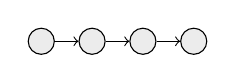
\begin{tikzpicture}[node distance=0.3cm]
        \node[mini world] (a) {};
        \node[mini world] (b) [right=of a] {};
        \node[mini world] (c) [right=of b] {};
        \node[mini world] (d) [right=of c] {};
        \path[->] (a) edge (b);
        \path[->] (b) edge (c);
        \path[->] (c) edge (d);
    \end{tikzpicture}
};

\draw [->, >=stealth', shorten >=7pt, shorten <=7pt] (A.east) to (M.west);
\draw [->, >=stealth', shorten >=7pt, shorten <=7pt] (B.east) to (M.west);
\draw [->, >=stealth', shorten >=7pt, shorten <=7pt] (M.east) to node[above left]{\footnotesize \color{OliveGreen} TRUE} (C.west);
\draw [->, >=stealth', shorten >=7pt, shorten <=7pt] (M.east) to node[below left]{\footnotesize \color{Red} FALSE} (D.west);

\end{tikzpicture}
\caption{The Model Checking Structure adapted from E. Clarke \cite{Clarke:2008:BMC:1423535.1423536}}
\label{fig:mcs}
\end{figure}

Model checking is capable to verify both \textit{safety} and \textit{liveness} properties of a software in sightly different manner \cite{4544862}. Safety properties means nothing bad happens in the program execution, such as arithmetic overflow, buffer overflow, or NULL dereference, which can be verified by proving the unreachability of these states. Liveness properties means something good eventually happens. This can be proved by showing that a program fulfilled its functional specifications or it simply guaranteed termination at the end. A program can be claimed as verified while all the given properties are satisfied by the given model. This technique is precise as all reachable states have been examined, however, the number of states can grows exponentially along with the complexity of the program \cite{Clarke:2001:BMC:510986.510987, biere2003bounded}. The state explosion problem becomes a major weakness of such techniques. In the history of model checking, several techniques have been applied in order to increase the capacity of the exploration states, for examples, some efficient graph traversal techniques, the symbolic representation, Binary Decision Diagrams (BDDs), and so on. During the 1990s, the combination of symbolic model checking with BDDs was proposed and continuously be improved. While symbolic representation encode sets of states into Boolean functions and BBDs further transform the boolean formulas as a canonical form, it allows transitions can be applied to a set of states directly instead of an individual state in each iterations. Because of the use of BDDs and some abstraction techniques, the capacity level has been improved, and model checking has also been applied on some realistic systems. However, the size of BDDs can grow exponentially, which becomes a bottleneck of verification as the efficiency and capability are restricted, and it is still not enough to carry out a full verification to meet the industrial needs.

\section{Bounded Model Checking} \label{sec:bmc}
% should be useful \cite{Clarke:2001:BMC:510986.510987}
Bounded Model Checking (BMC) based on Boolean Satisfiability (SAT) was introduced by A. Biere et al. in 1999\cite{biere2003bounded}. Although it does not overcome the entire complexity weakness of model checking, it is more capable to verify different circumstances comparing with using the BDD-based techniques. While BMC only cover the execution paths within the user-defined bound, the properties beyond the bound will not be verified. Instead of proving "\textit{all reachable states satisfies the property $p$}", \textbf{AG}$p$, is true directly, the formula can also be checked in its negation by showing that "\textit{there exists a reachable state violates the property $p$}", \textbf{EF}$\neg p$, is false. This means that a counterexample of \textbf{AG}$p$ is a witness of \textbf{EF}$\neg p$ \cite{Clarke:2001:BMC:510986.510987}. Hence, the concept of BMC is to check the negation of given property $\varphi$ up to a given depth $k$, in order to find a witness for showing such a violation exists \cite{7423219}, shown in the Figure~\ref{fig:bmcm} below. 

% Consider we have a state transition model $M$, a property $\varphi$ and a constant bound of $k$ iterations, the BMC problem becomes whether a witness within $k$ steps exists such that the property $\neg P$ is satisfied by the unrolled transition model $M$,. 

\begin{figure}[!h]
\centering


\begin{tikzpicture}[node distance=1cm]
    \node[world] (a) [label={[name=s0]below:$s_0$}, label={[name=p0]above:$\neg\varphi_0$}] {};
    \node[world] (b) [right=of a, label=below:{$s_1$}, label=above:{$\neg\varphi_1$}] {};
    \node[world] (c) [right=of b, label=below:{$s_2$}, label=above:{$\neg\varphi_2$}] {};
    \node[world] (d) [right=of c, label={[name=sk-1]below:$s_{k-1}$}, label=above:{$\neg\varphi_{k-1}$}] {};
    \node[world] (e) [right=of d, label={[name=sk]below:$s_k$}, label={[name=pk]above:$\neg\varphi_k$}] {};
    \path[->] (a) edge node [midway, above] {$\lor$} (b);
    \path[->] (b) edge node [midway, above] {$\lor$} (c);
    \path[loosely dotted] (c) edge node [midway, above] {$\lor$} (d);
    \path[->] (d) edge node [near end, above] {$\lor$} (e);
    
    \node (stm) [left=of s0, align=right] {state of \\ transition model};
    \node (p) [right=of pk, align=right] {property};
    \node (bound) [right=of sk, align=right] {bound};
    \path[dashed, ->] (stm) edge (s0);
    \path[dashed, ->] (p) edge (pk);
    \path[dashed, ->] (bound) edge (sk);
    
    \draw[red,thick,dotted, rounded corners] ($(p0.north west)+(-0.15,0.15)$) rectangle ($(sk-1.south east)+(0.15,-0.15)$) node[black, below left] {counterexample trace};
\end{tikzpicture}

\caption{The idea behind Bound Model Checking adapted from H. Rocha et al. \cite{7423219}}
\label{fig:bmcm}
\end{figure}

In addition, such a boolean formula can be reduced as a SAT problem and hence it can be solved by a SAT solver \cite{biere2003bounded, 1_sagiv_2015}. The advantage of replacing BDDs with SAT is that the exponential growth of space in BDDs can be avoid, and also smart depth first search can be applied to reduce the memory consumption when using breadth first search in BDDs. 

Sometimes there is a chance of missing bugs in the verification, due to the given bound does not cover all the possible execution paths, hence choosing an appropriate bound is fundamental to minimise such a chance. In practise, it is suggested to begin with a smaller length $k$, and then continue with a larger one if there is no error is found. Nevertheless, the verification result is promising while a counterexample can locate exactly where the violation is and all bugs within the bound are guaranteed to be found. Even when the property is not allow for proving the correctness, BMC is still useful and reliable for finding counterexamples. Because of such improvements and this impressive feature, BMC based on SAT has been successfully used in the formal verification of industrial practises. 

% Hence, even if there is infinite number of states, BMC can still be applied by bounding the number of exploring states. Concerning the coverage of the verification, the bounded can lead to an verification as bugs may exist beyond the bound. Nevertheless, all bugs within the bound are guaranteed to be identified. 

% Not done
\section{C Bounded Model Checker (CBMC)} \label{sec:cbmc}
CBMC \footnote{The CBMC Homepage: http://www.cprover.org/cbmc/}, despite its name, is a bound model checking tool for the formal verification of ANSI-C programs using SAT solvers developed by D. Kroening et al. \cite{ckl2004}. It aims at reasoning about the safety properties of low level ANSI-C implementation as many safety-critical software are written in such low level languages. 

\subsection{Ready for verifying a program}
In order to analysis a given C/C++ code, CBMC will first reduce the model checking problem to a validity of bit vector equation problem by translating the program statement into an static single assignment (SSA) form \cite{ckl2004, Clarke:2003:HVU:1119772.1119831}. The translation consists of three main procedures described as follows: 

\paragraph{Program translation} Suppose the ANSI-C program has been preprocessed already. The program will be translated into a consistent form, which is only consists of \code{if}, \code{while}, \code{goto} statements and simple assignments without any side effects by applying some semantics equivalent replacements listed below:

\begin{table}[H]
\centering
\begin{tabular}{| p{.4\textwidth} | c | p{.45\textwidth} |} 
\hline
Original instructions & $\to$ & Transformed statements \\
\hline
\hline
\code{break}, \code{continue}, \code{return}  & $\to$ & \code{goto} \\
\hline
\code{switch}, \code{case}  & $\to$ & \code{if}, \code{goto} \\
\hline
\code{for}, \code{do while}  & $\to$ & \code{while} \\
\hline
\textit{Side effects}, i.e., function calls and pre- and post-increment operators & $\to$ & \textit{Assignments} using auxiliary variables \\
e.g. \code{x=j+(i++);} & $\to$ & \code{tmp_i=i; i=i+1; x=j+tmp_i;} \\ 
\hline
\end{tabular}
\caption{Program translation process descripted in \cite{Clarke:2003:HVU:1119772.1119831}}
\end{table}

\paragraph{Loop unwinding} In order to model the computation up to a given depth, loops are necessary to be unwound into a fixed number of iterations. This can be done by repeating the loop body with certain amounts of copies. While each copy is guarded by an \code{if} statement with the same condition as the loop, it is prepared for the case that less iterations are required for the loop. In addition, an assertion with the negated condition can be added after the last copy, which can ensure that the loop does not require more iterations by using \code{--unwinding-assertions} option in CBMC. This
is essential for showing that whether the unwinding bound is large enough to model the program behaviour. Note that, after the program translation process above, loops can be constructed by using \code{while} statements, recursive function calls, and \code{goto} statements. We use \code{while} as an example below: 

% $$\code{while(cond) instr}; \to \code{if(cond) {instr; while(cond) instr};}$$, such that

% \smallskip
% \noindent
\begin{figure}[H]
\centering
{
\begin{minipage}{.2\textwidth}
\begin{minted}[fontsize=\footnotesize]{c}
while(cond) {
    instr;
}    
\end{minted}
\end{minipage}
\begin{minipage}[]{.05\textwidth}
$\to$
\end{minipage}
\begin{minipage}[]{.5\textwidth}
\begin{minted}[fontsize=\footnotesize]{c}
if(cond) {
    instr; /** 1st copy **/
    if(cond) {
        instr; /** 2nd copy **/
            ...
            if(cond) {
                instr; /** kth copy **/
                
                /** unwinding assertion **/
                assert(!cond)]; 
            }
    }
}    
\end{minted}
\end{minipage}
}
\caption[The LOF caption]{Loop unwinding for $k$ times with unwinding assertion adapted from CPROVER tutorials \protect\footnotemark}
\end{figure}
\footnotetext{The CPROVER manual: http://www.cprover.org/cprover-manual/}
% \bigskip

\paragraph{Variable Renaming}
After the previous operations, the program, containing \code{if} statements, assignments, assertions, \code{goto} instructions and labels only, is ready to be transformed into SSA form by using pointer analysis. The transformation is demostrated by the simple example below:

\begin{figure}[H]
\centering
{
\begin{minipage}{.2\textwidth}
\begin{minted}[fontsize=\footnotesize]{c}
x=x+y;
if(x!=1)
    x=2;
else
    x++;

assert(x<=3);
\end{minted}
\end{minipage}
\begin{minipage}[]{.05\textwidth}
$\to$
\end{minipage}
\begin{minipage}[]{.2\textwidth}
\begin{minted}[fontsize=\footnotesize, escapeinside=||,mathescape=true]{c}
x|$_1$|=x|$_0$|+y|$_0$|;
if(x|$_1$|!=1)
    x|$_2$|=2;
else
    x|$_3$|=x|$_1$|+1;
    
x|$_4$|=(x|$_1$|!=1)?x|$_2$|:x|$_3$|;
assert(x|$_4$|<=3);
\end{minted}
\end{minipage}
\begin{minipage}[]{.05\textwidth}
$\to$
\end{minipage}
\begin{minipage}[]{.35\textwidth}
\begin{align*}
    C \coloneqq{}& \code{x}_1\code{=x}_0\code{+y}_0 \land \\
    &  \code{x}_2\code{=2} \land \\
    &  \code{x}_3\code{=x}_1\code{+1} \land \\
    &  \code{x}_4\code{=(x}_1\code{!=1)?x}_2\code{:x}_3 \\
    P \coloneqq{}& \code{x}_4\leq\code{3} \\
\end{align*}
\end{minipage}
}
\caption[The LOF caption]{SSA form transformation adapted from \cite{ckl2004, Clarke:2003:HVU:1119772.1119831}}
\end{figure}

The procedure above renames all variables with states to ensure that each variable is fresh and will only be assigned once. As a result, the program can be viewed as a set of constraints and two bit-vector equations, constraints $C$ and properties $P$, can be produced accordingly. Hence, the property can now be verified by converting $C \land \neg P$ into Conjunctive Normal Form (CNF) through a SAT solver. Once the equation is \textit{satisfiable} which means a violation of the given property is found, otherwise, the property holds when the equation is \textit{unsatisfiable}. 

\subsection{Assumption \& Assertion}
As mentioned above, CBMC considers the verification conditions as a pair of bit-vector equations, constraints $C$ and properties $P$, which is specified by using \textit{assumption} (\code{__CPROVER_assume()}) and \textit{assertion} (\code{__CPROVER_assert()}) statement respectively. The \code{__CPROVER_assert()} statement takes a Boolean condition, which is an ANSI-C logic expression, and a string description as arguments. CBMC will check the given condition holds for all executions. The description is useful for locating the violated assertion. The \code{__CPROVER_assuem()} statement will also takes a Boolean expression, which is used to restrict the program traces exploration. The program trace examination will be aborted while the given assumption is false.

\subsection{Non-Determinism}
Non-deterministic choice functions is supported in CBMC by declaring \code{nondet_} as the prefix of their names and it is usefully for modelling the user inputs. The range of the generated values depends on the return type of the function and also the restriction given by the corresponding assumptions. 

\subsection{Automatic Verification} 
Concerning to the verification on safety properties, CBMC takes care of a widely range of program behaviour regarding to such properties, including dynamic allocations using \code{malloc()} and \code{free()}, buffer overflow, pointer safety, arithmetic overflow, user-defined assertions, etc. Moreover, by enabling CBMC with different options, the verification condition generator of CBMC will automatically generate the safety conditions respectively, which allows the above verifications become fully automated. The options of supported build-in safety check are as follows: \code{--divided-by-zero-check}, \code{--bounds-check}, \code{--pointer-check},  \code{--memory-leak-check}, and \code{--signed-overflow-check} as well as \code{--unsigned-overflow-check}. Because of the advantage of being automated and the verification capability, CBMC has been widely used in a variety of applications, such as error explanation, verifying embedded programs, finding security bugs in windows binaries, etc.

% SAT-based Bounded Software Model Checking for Embedded Software: A Case Study
% High maturity of CBMC:
% CBMC can analyze target ANSI C code as it is and generate sound verification result (modulo user- given loop upper bounds). In contrast, other software model checkers targeting C code such as Blast [4] and CPAChecker [5] have limitations in analyzing complex target C code in practice (for example, Blast does not analyze array operations correctly [20]). In addition, CBMC has been developed more than 10 years and become more reliable than other research prototype tools of short development history.

% \section{Overview of the TLS/SSL}

\section{Overview of s2n}
s2n \cite{3_the_s2n_user_manual, 4_introducing_s2n} is an open-source implementation of the TLS/SSL protocols that was released in late June 2015 by the Amazon Security Labs. It is designed with the concern of security, reviewability, ease of use and efficiency. It can support various version of the TLS/SSL protocols, such as SSLv3, TLS1.0-1.2, with different cipher suites. The implementation of s2n is only around 6,000 lines of C99 code as it relies on OpenSSL or other its forks for handling the low-level cryptographic computation of the TLS protocol. Comparing with the implementation of OpenSSL which needs about 70,000 lines of code to implement the protocol. This makes s2n easier to be reviewed, indeed, Amazon also announced that three external security evaluations and penetration tests had been done on s2n at that time. 


% Show wt CBMC / Bounded model checking can do

\section{Related Work}
The use of model checking technique for automated formal verification of software has been presented and widely researched over the last couples of decades. In this section, we discuss some practical applications and experiences of applying model checking techniques on security audit and assurance. It is important to learn from the successful cases from others in order to observe how the model checking is being used effectively and what kind of effect it has contributed to the development process and the overall quality.

\subsection{Formal software verification techniques}
There are numerous formal verification techniques available for software verification. Each of them is designed for a particular purpose. We discuss those techniques which are highly researched or presented recently.
% A Survey of Automated Techniques for Formal Software Verification
A survey that conducted by V. D'Silva et al. \cite{4544862} gave a detailed overview of three main automatic formal verification techniques, and brought out their strengths and weaknesses for applying to practical problems. The three techniques are: 1) Static Analysis, 2) Model Checking, and 3) Bounded Model Checking. We discuss each of them in detail below.

% What is it
% How it works
% Limitation?
% Advantages.
% Compare with BMC
% Some statictis

% Comparing Model Checking and Static Program Analysis: A Case Study in Error Detection Approaches
\paragraph{Static analysis} generally refers to a family of techniques for determining the run-time properties of a program without executing it. Static analysis is able to indicate run-time errors automatically at compilation time without any code instrumentation or user interaction. Therefore, these techniques are commonly used in compiler optimisation. In term of software verification, the soundness of an analysis relies on the approximation, which becomes a limitation to static analysis. As the undecidability of static analysis problems, it is not possible to come up with an approximation that produces no false positive and no false negative detections. It uses some simple predefined fact for showing the absence of simple errors, such as no assertion violation, no arithmetic overflow, and no exceed of array bounds, efficiently. However, it is difficult to generate counterexamples, due to the precision loss during the analysis which is a significant trade-off for efficiency.

In contrast to static analysis, model checking is more precise as it can prove more complicated properties and provides counterexamples once a bug is found. The above statements are supported by the experimental result conducted by K. Vorobyov and P. Krishnan \cite{vorobyov2010comparing}. The experiment compares the verification result of static program analysis with the one of model checking by applying Parfait and CBMC respectively on some benchmarked code base. By configuring CBMC to focus on particular types of error, it showed a high accuracy rate (97\% overall true positive detections, and found about 19\% more bugs), whereas only 77\% with Parfait. Moreover, both of them reported a 0\% false positive detections, which is common for model checking and a specific design to minimise it for static program analysis. However, model checking is much more expensive with respect to computation time and memory usage, as it reached the memory limit in the experiment. The study further concluded that: 1) scalability can be a problem for model checking a large size code base, such as an operating system, and 2) an insufficient unwinding was one of the reasons for false negative detections of CBMC.

\paragraph{Model Checking} is a technique for verifying the correctness of a finite-state system as mentioned in Section~\ref{sec:mc}. It computes the run-time states of the software without actually running the program. Each reachable state is examined whether a correctness property holds. If such an execution path violating any of the properties is found, a counterexample is formed. This process is guaranteed to terminate only if there are finite states. This technique is frequently used on verifying the safety properties of device drivers and systems code. However, it is easy to run into a state space explosion problem while analysing a medium sized code bases \cite{Yeolekar2013}. Even with the help of SAT or SMT solver and some abstraction techniques, model checking is hard to scale up to the size level that static analysis does. 

\paragraph{Bounded Model Checking} is a complementary technique to model checking with an upper bound of the number for explored state as mentioned in Section~\ref{sec:bmc}. It unrolls the transition operations for $k$ times and combines the properties to form a propositional formula, which is solvable by a SAT solver. The formula is satisfiable as long as the property is violated by a trace of length $k$. Such technique is sound for the execution paths up to the specified length $k$, while a bug can exist beyond the bound. Although it may result in an inconclusive outcome, BMC is still a great successful technique for finding bugs, as well as proving the liveness and safety properties by applying in different manner. V. D'Silva et al. \cite{4544862} further concluded that bounded model checking is the best technique to find shallow bugs comping with static analysis and model checking, and is able to provide a complete counterexample trace once a bug is found. However, the completeness is not guaranteed if the program contains deep loops.

% very useful paper, about abstraction
% The concept of dynamic analysis
\paragraph{Dynamic analysis} is a technique to analyse the run-time proprieties by executing a program, which is in contrast to static analysis. It is not able to prove a particular property holds, but nevertheless it is useful for detecting violations of properties \cite{Ball:1999:CDA:318774.318944} and able to scale to large-size code bases. A. Yeolekar and D. Unadkat \cite{Yeolekar2013} presented a counterexample-guided abstraction refinement (CEGAR) based technique by utilising dynamic analysis to overcome the scalability limitation of model checking. Dynamic inference is used to guess invariants and refine the abstraction from spurious counterexamples, thus a better precision of the abstraction and an accelerated loop refinement are achieved in their experiment.

% Concolic Testing of the Multi-sector Read Operation for Flash Memory File System
% comparing concolic testing with model checking
\paragraph{Concolic testing} is a hybrid software verification technique joining symbolic static analysis and concrete dynamic analysis, which is able to generate test cases automatically and to examine execution paths exhaustively. M. Kim et al. \cite{Kim:2009:CTM:1693660.1693677} conducted an experiment on concolic testing to analyse the multi-sector read operation for a flash memory, and summarised its advantages and weaknesses compared to model checking techniques. Concolic testing algorithm in general consists of five steps: 1) Instrumentation, 2) Concrete execution, 3) Symbolic execution, 4) Deciding the next execution path, and 5) Choosing the next input values. As the symbolic execution preforms along the concrete execution path, no false alarms will be produced. Once the path formulas are not able to be solved by a constraint solver, some symbolic constraints will be simplified by replacing some of the symbolic values with concrete value. This may leads to an incomplete coverage. The experimental result showed it had a better applicability and lower memory usage. However, the study also reflected that concolic testing is a time-consuming method as time will be wasted on generating invalid test cases in a complex environment model. %Concolic testing can analyse a software with underlying binary libraries without any manual abstraction, which is necessary for model checking. 
Concolic testing can be a good choice for finding bugs, but not for demonstrating program correctness. Model checking generally provides high accuracy and a better performance of the verification than concolic testing, which is essential for verifying critical software.

\subsection{Software Verification approaches through MC}

% Traditional testing vs Abstract testing.
% Bridging the gap between test cases and requirements by abstract testing
\paragraph{Abstract testing} is a software testing approach proposed by F. Merz et al. \cite{Merz:2015:BGT:2837773.2837824}, which focuses on the relation between requirements and the corresponding test cases in order to replace the traditional test cases by an abstract one. Each abstract test cases is derived form the requirements and formulated into assumption and assertion statements on the source code level, which is often a one to one relation. Assumption and assertion statements are the constraints encoding the preconditions and postconditions respectively. Setting up these constraints for the testing environment with respect to non-deterministic values, rather using concrete values. Hence, an abstract test case is possible to represent a large number of concrete test cases, which can remarkably simplify the test cases generation and maintenance process. The experimental study showed that abstract testing is more capable and efficient to discover underlying bugs than traditional software testing. Moreover, the performance of CBMC is promising with less than 20s runtime on average for an abstract test case, which is suitable for agile-like development process. Once there is a change of requirement, it is easily and directly visible to the corresponding abstract test cases.

%  ********** may be related
% Unit Testing of Flash Memory Device Driver through a SAT-Based Model Checker
Besides the incomplete coverage of conventional testing stated above, M. Kim et al. \cite{4639323, Kim:2008:FVF:1429078.1429092, 5510242} also mentioned that once a violation is detected, it still require a large amount of human effort to locate where the violation occurred by replaying the scenario and tracing the execution step-by-step. Hence, model checking techniques is well-suited to overcoming these weaknesses of conventional testing method through exhaustive analyses. This study applied SAT-based bounded model checking technique to verify the functional correctness and increase the reliability of the device driver software for Samsung's OneNAND\textsuperscript{TM} flash memory. In order to extract the code level properties, the study also suggested a top-down approach to identify the properties from several design documents, such as software requirement specifications, architecture design specifications, and detailed design specifications. It demonstrated a practical way on how the functional correctness properties can be extracted from the real world environment. By replacing the conventional testing with constraint-based exhaustive testing, which is the same as abstract testing above, CBMC achieved a great success in the experiment that discovered some bugs including incomplete exceptions handling and logical bugs. This promising result shows that model checking techniques are mature enough to be applied on verifying an industrial level software.

% Unit Testing of Flash Memory Device Driver through a SAT-Based Model Checker
% One advantage of SAT-based model checking is that a target C code can be analysed directly without an abstract model, thereby enabling automated and bit-level accurate verification. 
% Software requirement specifications (SRS), Architecture design specifications (ADS), Detailed design specifications (DDS)

% Property-based Code Slicing for Efficient Verification of OSEK/VDX Operating Systems
% very useful paper and also about CBMC
\paragraph{Property-based code slicing}
Despite the fact that model checking is a powerful technique, it often requires more knowledge and cost than testing. In order to reduce the cost while maintain comprehensiveness, M. Park et al. \cite{DBLP:journals/corr/abs-1301-0042} proposed an approach that consists of three strategies: 1) property-based environment generation, 2) property-based abstraction, and 3) collaborative verification using model checking and testing. The study applied it to verify the Trampoline operating system. The result showed that the approach is able to reduce the verification cost by scaling down the target code, and to simplify the analysis process by localising the verification activity.

% working on it.

% property-based environment generation and model extraction techniques using static code analysis, which can be applied to both model checking and testing. Comparative experiments using random testing and model checking for the verification of assertions in the Trampoline kernel code show how our environment generation and abstraction approach can be utilised for efficient fault detection. 

% Testing is insufficient for identifying subtle issues due to its optimistic incompleteness.

% Model checking is a powerful technique that supports comprehensiveness, and is thus suitable for the verification of safety-critical systems. However, it generally requires more knowledge and cost more than testing.

\paragraph{False positive elimination}
Software verification based on abstract interpretation is scalable for verifying industrial level code bases, but imprecise. Many spurious errors are generated as the abstract interpretation over-approximated the execution traces than the program can actually perform. Manual investigation is needed to review each error, such manual efforts are costly to the development process. To overcome this problem, 
% Reducing false positive
% Reducing False Positives by Combining Abstract Interpretation and Bounded Model Checking
H. Post et al. \cite{4639322} and P. Darke et al. \cite{Kumar:2013:PRA:2491411.2494569} integrate model checking to reduce the number of false positive generated by the static analysis tools. The experimental result shows that 69\% of warnings have been successfully removed by CBMC. 

% Reducing False Positives by Combining Abstract Interpretation and Bounded Model Checking
% The study shows that CBMC can generally provide more counter-example than SATABS. Abstract interpretation uses an over-approximation on the set of possible execution trace. i.e., it considers more program execution paths than the program can actually perform. Introduce false positives.

% doi not found, false positive elimination
% Efficient Elimination of False Positives Using Bounded Model Checking
Another study by T. Muske et al \cite{tukaram2013efficient} points out the above approach could involve numerous verifications, and further proposes an approach consisting of three techniques to achieve a faster false positives elimination. By avoiding redundant equivalent assertions, results in a 60\% accelerated false positives elimination. 

% identify an assertion as being equivalent to an other assertion thus avoiding its verification. Then, tries to identify and skip a class of assertion verifications that will not eliminate a false positive.

% Software verification using abstract interpretation is scalable but imprecise. Model checking is precise in verifying a property but not scalable. Often, these two techniques are combined to achieve better precision.

% On the Formal Verification of Component-based Embedded Operating Systems
% system level verification - isolation of components for modular verification
\paragraph{Aspect-oriented programming technique} M. Ludwich and A. Frohlich \cite{Ludwich:2013:FVC:2433140.2433148} introduced an approach to formally verify both \textit{functional correctness} and \textit{safety properties} of embedded operating system components. Such components are supposed to be shifted between different domains, therefore, the implementation of formal verification must also be domain-independent. The study proposed a corresponding strategy that consists of three main steps: 1) creating contracts for each components that to be verified , 2) implementing such components with the corresponding contracts accordingly, and 3) performing software bounded model checking to verify whether the implementation of components respect to their contracts. The benefits of keeping the specification and implementation close to each other is that any violations in the implementation can be detected at the early stage of development. However, this may introduce an extra run-time overhead to its instances. Hence, those contracts should be partially eliminated from the implementations beyond the verification stage. The experiment made used of aspect-oriented programming technique to achieve this purpose, and further facilitate a modular verification by isolation different components. Note that components isolation is not suitable for verifying a monolithic design. More importantly, the experiment also demonstrated that the functional correctness and safety properties can be verified by the contracts captured from requirements and those properties generated by the model checker respectively. This approach is a kind of white box testing and is more suitable to carry out at the early stage or during the development.

% How Verified is My Code? Falsification-Driven Verification (T)
\paragraph{Falsification-Driven Verification} A. Groce et al. \cite{7372062} stated the idea of a "verification successful" in model checking or even theorem proving can be a sign of insufficient verification properties. In order to gain more knowledge of the meaning behind "successful" results, the study proposed a falsification-driven methodology that adapts mutation testing to show the weakness of current specification. Mutate both the harness and the program with a small syntactic change assuming a good test suit should be able to detect a bug introduced by such a change. Hence, the mutation kill rate can act as a measurement unit of the accuracy rate and correctness of a harness. As a better harness should able to detect more errors from the implementation. This approach is useful for ensuring the quality of harnesses, thus a more reliable verification. However, it requires many manual efforts to verify and examine the mutants while some of them can be semantically equivalent. It would be suitable for developers who are not familiar with formal verification but intend to verify a system.

% On the Formal Verification of Component-based Embedded Operating Systems
% Moreover, they demonstrate the approach causes no run-time overhead, since the adopted Software Model Checking techniques are deployed at compile-time. The functional correctness properties of a component are expressed by a contract containing assertions that represent class invariants, pre, and postconditions for each method declared in the component's interface. The safety properties are meant to be automatically generated by model checker.


% A contract is composed by the invariants of the class that defines the component and by a set of pre and postconditions. Class invariants are defined as a set of assertions that are always true for all instances of that class. The preconditions of a method define a set of assertions that must be true in case the method invocation terminated normally (ie. without triggering exceptions, which have not yet been addressed in our approach.) Pre and postcondition assertions can reason about the method's parameters, return value, and object state.

% Bridging the gap between test cases and requirements by abstract testing
% The havoc() procedure call in the example sets some global vari- ables to undefined (non-deterministic) values.

% \begin{itemize}
%     \item Software testing only consists of few selected cased for checking the correctness, which is sound but not complete.
%     \item Abstraction based verification techniques covers all possible input spaces, which is complete but may cause false positive.
%     \item Bounded Model Checking is sound, but only execution paths up to the specified length are checked; therefor not complete.
%     \item BMC with large enough bound is sound and complete.
% \end{itemize}


% no really helpful - configuration lifting
% Configuration Lifting: Verification meets Software Configuration
\paragraph{Configuration lifting} is a specification analysis technique presented by
H. Post and C. Sinz \cite{4639338}, which transforms all variants into a meta-program and facilitates the following specification analysis in three different domains: 1) inconsistencies within a feature model, 2) inconsistencies between the feature model and their implementations, and also 3) the coverage of run-time errors in all product variants. The study demonstrated the technique on verifying Linux kernel and device driver, which successfully found two bugs in the kernel configuration system. The experimental result showed that this technique is able to apply on a large size system included more than 4600 features and model checking on the meta-program provides a significant speed-up compared with traditional enumeration based analysis.

% Semiformal Verification of Embedded Software in Medical Devices Considering - Stringent Hardware Constraints
\paragraph{Other approaches} L. Cordeiro et al. \cite{5066674} propose a semi-formal verification approach combined dynamic and static verification to stress and cover the state spaces of embedded software exhaustively, in order to improve the coverage and reduces the verification time. This approach allows developers to reason both the functional and temporal properties quantitatively to guarantee the timeliness and correctness of the design. The experimental result shows that model checkers have  limitation to specify more complex temporal properties and state space explosion problem.

\subsection{Practical software verification}
Software verification can generally be categorised into two main purposes: 1) hunting bugs, and 2) proving the program correctness. Below are several case studies which are making good use of the model checking are discussed below:

\subsubsection{Hunting bugs}
% Towards Improving Software Security using Language Engineering and mbeddr C
M. Voelter et al.\cite{Voelter:2015:TIS:2846696.2846698} took several well-know bugs as examples to show how the modular extension of the C programming language can improve software security. One of the examples is the Heartbleed bug in OpenSSL TLS mentioned in Section~\ref{sec:heartbleed bug}. By constructing a simple harness and a message with a nondeterministic data buffer, CBMC is able to identify the failure in a short period. This is a great demonstration of the importance of formal verification in the software development. 

% SAT-based Bounded Software Model Checking for Embedded Software: A Case Study
Another remarkable case study presented by Y. Kim and M. Kim \cite{7091291} has successfully detected four hidden bugs in an embedded software, lazybox ls, using CBMC. This study highlighted the pivot of loops analysis, determining the minimum iterations to exit a loop, to avoid false negative detections in practice. As an accurate unwinding loop bound can minimise the chances of missing bugs, state explosion, and execution timeout. The experiment also showed the effectiveness of using such model checking technique and its limitation on the loop analysis. 

% Using Model Checking to Find Serious File System Errors
There is a case study conducted by J. Yang et al. \cite{Yang:2006:UMC:1189256.1189259} demonstrated a systematical way to model check three widely-used and heavily-tested file systems. Two classes of checks are suggested: 1) generic checks for those general properties should hold at any point, and 2) consistency checks for the functional properties that the file system specified. Concerning the complexity of such file systems, it is impractical to be fully tested in the traditional way as there could be an exponential number of test cases for checking the recovery mechanism. Model checking make use of several state-reducing techniques, which makes it capable to explore such vast state spaces efficiently. As a result, 32 serious bugs are found during the experiment.

\subsubsection{Proving correctness}
% very useful experiment
% Verifying Code and Its Optimizations: An Experience Report
An experience report presented by R. Metta \cite{Metta:2011:VCO:2004685.2005455} described their experience in verifying the correctness of a 200-line implementation of Cyclic Redundancy Check. The study indicated that sometime the specification and verification process can hardly be automated and required intense human efforts even for such a small code bases. It is hard to scale up if such a program containing huge loops. The authors further suggested a bottom-up approach to verify the correctness of each functions independently through CBMC first, and then to verify the correctness of the loop through an induction manually using CBMC. 

% Verification of Safety-Critical Systems: A Case Study Report on Using Modern Model Checking Tools
A. J{\"a}{\"a}skel{\"a}i et al. \cite{jskelinen_et_al:OASIcs:2012:3589} verified the implementation of the 2003 voting scheme in a systematic capability 3 level shutdown system through model checking. The experiment is conducted in two stages: 1) refine and translate the requirements into pseudo code directly for a preliminary verification, and then move on to 2) verify the actual implementation of the voting scheme. The study concluded in several suggestions for using model checking techniques. Beginning with some simple test cases can help to understand how to give precise and effective assertions before jumping into those complicated properties. Fault seeding techniques is recommended for inexperienced users in order to check the correctness of assertions by introducing violation to the corresponding properties. 
% done

% Automated Verification for Functional and Relational Properties of Voting Rules
Another study conducted by B. Beckert et al. \cite{beckertBormerKirsten2016} verified the functional and relational properties of voting rules, and demonstrated the effectiveness of using bounded model checking and deductive verification. Moreover, it also showed that the verification effort can be greatly reduced by using symmetry properties. 

% can be very accurate, but it requires certain times and memory space for exploring the possible states.
F. Werner and D. Farago \cite{Werner2010CorrectnessOS} investigated CBMC to the domain of wireless sensor networks (WSNs) and proved that it is capable to perform automatic verification on a system about 21000 LoC. It showed that the scalability can be greatly improved by the proposed abstractions and simplification heuristics, with the --slice-formula option enabled. The study further concluded that CBMC with the abstractions and heuristics is powerful enough to verify large scale programs. 

\subsection{Model Checking tools}
\paragraph{CRUST} is a bounded verifier developed by J. Toman et al. \cite{7371997} combines exhaustive test generation and bounded model checking technique in order to detect memory safety errors. It will first generates a set of testing driver for those relevant APIs, converts the driver code from Rust to C, and then performs bounded model checking. With the help of exhaustive test generation, it is able to efficiently explore large input spaces and generated multiple test drivers for covering the input spaces as many as possible. CBMC is used as a back-end service for automated analysis. By evaluating data structures from Rust standard library, CRUST is capable to detect some memory safety bugs from it.

% % A Comparative Study of Software Model Checkers as Unit Testing Tools: An Industrial Case Study
% M. Kim et al. \cite{5510242} reported their experience in applying Blast and CBMC to testing the components of a storage platform software for flash memory.

% Significant additional efforts are required to create an abstract target model, which is not affordable for most industrial projects.



\subsection{Other applications}
There are several studies showing that model checking is applied to various usages, such as embedded software verification \cite{Cordeiro:2009:SBM:1747491.1747515, BK11}, cross-platform verification \cite{0fbeb641779543c98fb1d6ff2180664c}, sequentialisation-based verification \cite{6693139}, fault localisation \cite{Griesmayer:2007:AFL:1247747.1248089}, equivalence checking \cite{Lee2011}, cyber-physical system co-verification \cite{6649878}, and test-vector generation \cite{Angeletti2009}.


% \cite{5510242}
% There have been several studies in which an SMC was
% applied to various target systems such as automotive
% software [47], microcontroller programs [48], Linux device
% drivers [45], [46], file systems [52], network filters [13], a
% protocol stack [40], and server applications [41]. For a flash
% storage platform, which is our main target domain, one
% recent study [32] analyzes flash file systems as an effort of
% the mini-challenge [35]. However, the majority of verification
% research [36], [28], [11] on flash file systems focus on
% the specifications of the file system design and not on an
% actual instance of implementation.

% % not really helpful
% *T. Vortler et al. \cite{7195716} presented a verification framework for applications for the embedded system operating system Contiki, based on CBC, supporting interrupts.

% % not really helpful (something about partial reduction) - verifying sensor node using CBMC
% % D. Bucur and M. Kwiatkowska \cite{BK11}

% % not really helpful - but a bit about CBMC
% *B. Schlich and S. Kowalewski \cite{Schlich:2009:MCC:1569778.1569782} studied 14 tools and summarised the limitations for verifying embedded software.


% % Crowdsourcing Program Preconditions via a Classification Game
% % D. Fava et al. \cite{Fava:2016:CPP:2884781.2884865} used CBMC to generate the Invariant / check whether the precondition can cause the postcondition

% % % Seems not really helpful
% % I. Wenzel et al. \cite{0fbeb641779543c98fb1d6ff2180664c} 
% % only use CBMC for test data generation.

% % talked about memory safety
% *H. Post and W. K \cite{Post:2007:ISA:1770498.1770525} able to verify the memory safety of Linux drivers using CBMC.

% % Something about CBMC maybe useful
% *L. Cordeiro et al. \cite{Cordeiro:2009:SBM:1747491.1747515}
% CBMC has limitations due to the fact that the size of the propositional formulae increases significantly in the presence of large datapaths and high-level information is lost when the verification conditions are converted into propositional logic.


% \cite{Petrenko:2015:MTA:2744769.2747935}


% % Not very helpful, may be talk about some scale up problem & comparison with CBMC
% *P. Cousot et al. \cite{ousotEtAl10-FMSDC}


% % To the best of our knowledge, there is no work that considers .... As a result, our main contribution is ....
% \chapter{Approach and Hypothesis} % and System Implementation}

\section{Methodology}
% Proposed method.
In this project, we will verify the above software packages with the help of CBMC. The verification process can be separated into two stages. We will first conduct a low-level verification on them to ensure the memory safety with those generic checks provided by CMBC: 1) array bounds checks, 2) division by zero checks, 3) pointer checks, 4) memory leak checks, and 5) arithmetic over- and underflow checks.
% There are two different versions in order to support both signed types (e.g, int, long) and unsigned types (e.g, unsigned int, unsigned long). It will check whether there are any arithmetic over- and underflow on addition, subtraction, multiplication, division and negation operations. 

Then, we will go though the implementation and perform an application-level verification to ensure the correctness of the implementation. According to the approaches that the packages based on, we study the behaviour of each function, and then extract the specifications of them. Each specification consists of a pre-condition and a post-condition. A pre-condition stating the property required of the input is the responsibility of the environment. Hence, it is modelled by an assumption to assume the property holds before function has been executed. A post-condition describes the property of the output established by the function which is modelled by an assertion. Then, we inject these assumptions and assertions into each functions in order to capture the functional properties of the two applications. If all the properties pass the verification, then we can conclude that they are implemented correctly and memory safe.

\subsection{Top-down vs Bottom-up}
% reduce the false alarm.

\subsection{Liveness properties check}



\subsection{Specification Identification}

\subsection{Function call graph analysis}

\subsection{Stubbing}
A stub method is a method that just returns a simple but valid (though not necessarily correct) result.

\subsection{Loops analysis}
% A Survey of Automated Techniques for Formal Software Verification
This time is given by a bound on the maximum number of loop iterations and is usually computed via a simple syntactic analysis of loop structures. If the syntactic analysis fails, an iterative algorithm can be applied. First, a guess of the bound on the number of loop iterations is made. The loop is then unrolled up to this bound, as in Fig. 6, but with the assumption replaced by an assertion called an unwinding assertion. If the assertion is violated, there are paths in the program exceeding the bound, and a new guess for the bound is made [38], [83]. This method is applicable if the program (or its main loop body) has a run-time bound, which is highly desirable for many embedded applications.
\chapter{Experiment} \label{chpt:verification}

In this chapter, we describe our verification in details 

By the dependency analysis, we decide to verify the module of s2n in the following sequence (from the core part to the outer part)

All the verification result are summarised in Section~\ref{sec:verificationResult}

% % ***************************** s2n_blob

% \section{s2n\_blob Verification}
% The header file of \code{s2n_blob} is shown as follows. 
% \begin{listing}[ht]
% \inputminted[frame=single, breaklines, linenos, numbersep=5pt, tabsize=4, firstline=20, fontsize=\footnotesize]{c}{./contents/code/s2n_blob.h} %firstline=359, lastline=385, 
% \caption{The header file - s2n\_blob.h}
% \end{listing}

% There are 2 functions are declared in the header file, however, we found there is no method call that uses the function \code{s2n_blob_init()}. Alternatively, the \code{struct s2n_blob} always be initialised directly (line 14). According to the usage of these functions, we constructed a simple harness, shown as follows:

% \begin{listing}[ht]
% \inputminted[frame=single, breaklines, linenos, numbersep=5pt, tabsize=4, firstline=8, fontsize=\footnotesize]{c}{./contents/code/harness/s2n_blob_harness.c} %firstline=359, lastline=385, 
% \caption{The harness for \textit{s2n\_blob.h}}
% \end{listing}

% First, we create a \code{data} array with non-deterministic size (line 13) in order to model all possible size of data being wrapped in \code{struct s2n_blob}. Then, we apply the function \code{s2n_blob_zero()} to the initialised \code{struct s2n_blob}. Since there is no loop involved in the above harness, no loop bound analysis is needed.

% % *************************** s2n_mem
% \section{s2n\_mem Verification}

% There are 4 functions are declared in \textit{s2n\_mem.h}, which aim at handling the memory allocation of \code{struct s2n_blob}. As their names suggest, \code{s2n_alloc()} allocates a \code{s2n_blob} with the given size, \code{s2n_realloc()} reallocates the given \code{s2n_blob} with the given size and \code{s2n_free()} is used to reclaim the memory of the given \code{s2n_blob}. \code{s2n_mem_init()} initialises those environment variables related to memory allocation, for example, the system page size. 

% \begin{listing}[ht]
% \inputminted[frame=single, breaklines, linenos, numbersep=5pt, tabsize=4, firstline=22, fontsize=\footnotesize]{c}{./contents/code/s2n_mem.h} %firstline=359, lastline=385, 
% \caption{The header file - s2n\_mem.h}
% \end{listing}

% After studying the commonly practise of these functions, we created an corresponding harness with respect to the usage contracts of these functions. First, we prepare the environment with an uninitialised variable \code{s2n_blob} and a non-deterministic value as the size of the \code{s2n_blob} (line 11-14). Then, we initialise those s2n environment variables by using \code{s2n_mem_init()} (line 16) and finally we call the functions in the following sequence, \code{s2n_alloc()}, \code{s2n_realloc()} and \code{s2n_free()}. Similar to the case of \code{s2n_blob}, no loops is involved in these functions. Therefore, no loop bound analysis is needed as well.

% \begin{listing}[ht]
% \inputminted[frame=single, breaklines, linenos, numbersep=5pt, tabsize=4, firstline=9, fontsize=\footnotesize]{c}{./contents/code/harness/s2n_mem_harness.c} %firstline=359, lastline=385, 
% \caption{The harness for \textit{s2n\_mem.h}}
% \end{listing}


% \section{s2n\_stuffer Verification}

% \subsection{s2n\_stuffer}
% \subsection{s2n\_stuffer\_text}
% \subsection{s2n\_stuffer\_pem}
% \subsection{s2n\_stuffer\_base64}

\section{Tool Setup and Configuration}
\label{sec:tsc}


\section{Execution Environment}
\label{sec:ee}
% \subsection{Big / little endian}
% http://searchnetworking.techtarget.com/definition/big-endian-and-little-endian

% \section{Experiment Setup}
The machine configuration for the experiment is shown below:
\begin{table}[H]
    \centering
    \begin{tabular}{c|c}
        \hline
        \hline
        Item & Value \\
        \hline
        \hline
        Processor & 2.5 GHz Intel Core i7\\
        Memory & 16 GB 1600 MHz DDR3\\
        Disk & 500GB Apple SSD SM0512G Media\\
        OS & OS X 10.11.5\\
        CBMC Version & 5.4\\
        CBMC Github Commit ID & d031ccc0f8ec82495310c3268066dcde5bc18c59\\
        s2n Github Commit ID & 42d9daf1813e60b9c8ad235096309486e9fbfa05\\
        OpenSSL & 1.0.2i-dev \\
        \hline
        \hline
    \end{tabular}
    \caption{Machine Configuration}
    \label{tab:mc}
\end{table}

\section{CBMC Parameter Setting} \label{sec:cbmcps}

\section{Over-Approximation on ANSI-C Library}

\section{A detailed show case for show the verification procedure.}
\chapter{Experimental Evaluation}

\section{Achievement}
After the verification, we have successfully found two arithmetic overflow bugs in the s2n implementation and thus provided the corresponding solutions. The details are described in Section~\ref{seb:df} . A pull request\footnote{https://github.com/awslabs/s2n/pull/288} was submitted to the s2n Github repository and accepted by the Amazon s2n developers. They showed interest in our findings and wish to include the use of our techniques into their project. The details of the pull request and the conversation are shown in the screenshot in Figure~\ref{fig:achievement} below:

\begin{figure} [tp]
    \centering
    \includegraphics[width=\textwidth]{./contents/images/github-pullrequest.png}
    \caption{The screen capture of the accepted pull request and related conversations }
    \label{fig:achievement}
\end{figure}


\section{Detected Failures} \label{seb:df}
In this verification, CBMC reports 14 failures in seven different harnesses with all built-in checkers enabled, as mentioned in Section~\ref{sec:cbmcps}. By tracing the cause of the failures, we have discovered the similarity between the causes of failures and they can be concluded into four key issues: two bugs, one expected behaviour and one false alarm. Each key issue will be discussed in detail below:

\subsection{Unsigned Overflow on Memory Allocation}
An unsigned overflow failure is detected in the implementation of \code{s2n_realloc()} (line 56). The error trace and the implementation are listed in Listing~\ref{lst:eris2nRealloc} below:

\begin{listing}[ht]
\codeFromFile{text}{./contents/resources/verification-results/s2n_mem_harness-unsigned_overflow.txt}{detected-failures/s2n\_mem\_harness-unsigned\_overflow.txt}{}

\codeFromFile[firstline=50, lastline=  56]{c}{./contents/code/implementations/s2n_mem.c}{s2n/utils/s2n\_mem.c}{}
\caption{The error trace and the implementation of \code{s2n_realloc()}}
\label{lst:eris2nRealloc}
\end{listing}

Regarding the implementation of \code{s2n_realloc()}, we can see that there is no upper bounds check on the variable \code{size} before line 56. Since the value of \code{size} is given by the caller functions and it can be any possible value of type \code{uint32_t}, an unsigned overflow will occur at \code{(size + (page_size - 1))} operation (line 56) when the value of \code{size} is greater than \code{4,294,963,201}. Note that the value of \code{page_size} is commonly 4096 bytes (4KB), which is the default in s2n.
% This overflow can cause a sufficient memory allocation error as the value of \code{allocate}
This unsigned overflow can be prevented by rearranging the sequence of the calculation as shown below: (as compared to line 56 of Listing~\ref{lst:eris2nRealloc})

\begin{listing}[ht]
\codeFromFile[firstline=58, lastline=59]{c}{./contents/code/implementations/s2n_mem.c}{s2n/utils/s2n\_mem.c}{}
\caption{A fix for the implementation \code{s2n_realloc()}}
\label{lst:fis2nRealloc}
\end{listing}


\subsection{Signed Overflow on Type Conversion}
Another arithmetic overflow failure is detected on a type conversion in \code{s2n_connection_get_delay()} (line 379). The error trace and the detailed implementation are listed below: 

\begin{listing}[H]
\codeFromFile{text}{./contents/resources/verification-results/s2n_connection_gs_harness-signed_overflow.txt}{detected-failures/s2n\_connection\_gs\_harness-signed\_overflow.txt}{}

\codeFromFile[firstline=370, lastline=380]{c}{./contents/code/implementations/s2n_connection.c}{s2n/tls/s2n\_connection.c}{}
\caption{The error trace and the implementation of \code{s2n_connection_get_delay()}}
\end{listing}

This arithmetic overflow is due to the return type (\code{int64_t}) and the type of return variable (\code{uint64_t}) being inconsistent. Moreover, a signed integer overflow is an undefined behaviour in ANSI-C. As this is an API level function, the non-deterministic return value can lead to an unexpected behaviour in a third-party server implementation. This problem can be fixed with a correct return type of the function as shown below:

\begin{listing}[ht]
\codeFromFile[firstline=368, lastline=368]{c}{./contents/code/implementations/s2n_connection.c}{s2n/tls/s2n\_connection.c}{}
\caption{A fix for the implementation \code{s2n_connection_get_delay()}}
\end{listing}

\subsection{Memory Leaks on Error Exit}
Among 14 of the failures, five of them indicate memory leaks have occurred when the s2n process exit on error. According to the development guide, the error handling in s2n is done by the macros defined in \code{s2n_error.h} and \code{s2n_safety.h}, which return \code{-1} or \code{NULL} value directly in order to terminate the process immediately when an error exists. As a result, the process does not have a chance to deallocate the already allocated dynamic memory properly, and all of them remain in the heap after the process has been terminated. The suggested practice for error handling in s2n and the macros are shown in the following code snippets:

\begin{listing}[ht]
\codeFromFile[firstline=43, lastline=49]{c}{./contents/code/headers/s2n_safety.h}{s2n/utils/s2n\_safety.h}{}

\codeFromFile[firstline=28, lastline=29]{c}{./contents/code/headers/s2n_errno.h}{s2n/error/s2n\_errno.h}{}

\caption{The error handling and safety checking macros of s2n}
\end{listing}

The intention of the process is to guarantee its termination and in the case of error handling that is what the above macros are doing. Since most of the mainstream operating systems are able to reclaim all the heap memory allocated to the terminated process, therefore, this error handling behaviour is reasonable and does not count as a bug.


\subsection{Buffer over-read on \code{strlen()}}
In order to ensure maximum coverage of the harness, we allow all \code{char} arrays to carry every possible combination of values, even of those without any terminating character \code{'\0'}. However, three spurious warnings were detected on \code{strlen()} due to this approximation. Regarding the implementation of \code{strlen()}, it requires the input \code{char} array to be a string, which means an array must contain a terminating character \code{'\0'}.

\begin{listing}[ht]
\codeFromFile{c}{./contents/code/stubs/strlen.c}{cbmc/src/ansi-c/library/string.c}{}
\caption{The implementation of \code{strlen()} provided by CBMC}
\label{lst:strlen}
\end{listing}

This is the only criterion of using the function \code{strlen()} and we were not aware of that at the beginning. After a manual review on the verification result, we were able to trace this missing condition. A simple fix is done on the corresponding harnesses listed below. By introducing an assumption that the \code{char} array must carry at least one \code{'\0'} value, \code{s2n_stuffer_base64_harness.c} (line 15) and \code{s2n_connection_gs_harness.c} (line 16), the false alarms are removed.

\begin{listing}[ht]
\codeFromFile[firstline=14, lastline=15]{c}{./contents/code/harnesses/s2n_stuffer_base64_harness.c}{s2n-harness/module/s2n\_stuffer\_base64\_harness.c}{}

\codeFromFile[firstline=14, lastline=16]{c}{./contents/code/harnesses/s2n_connection_gs_harness.c}{s2n-harness/module/s2n\_connection\_gs\_harness.c}{}
\caption{Fixed the missing condition on 2 verification harnesses}
\end{listing}

\section{Loop Bounds Analysis Results}
There are over 50 different loops involved in the functions covered by the verification. 26 of whose LUBs are not able to be detected by CBMC automatically through syntactic analysis. We found most of the LUBs to be related to several particular sizes of data block, therefore there are some repeating LUBs, such as 17, 33, 49, 129 and 257. In Table~\ref{tab:lba}, it lists out the analysis results of all 26 loops in detail. The first four columns show the loop IDs given by CBMC, the filenames, the line numbers of where the loops are located, and LUBs of the loops respectively. The descriptions of the loops and the reasons for determining their corresponding LUBs are shown in the last column. 

For example, the loop \code{s2n_sslv3_mac_init.1} (the second row of Table~\ref{tab:lba}) assigns the standard padding value over the data block. Since the SSLv3 MAC function only supports two hash algorithms, SHA1 and MD5, their block sizes are 40 bytes and 48 bytes respectively. This loop iterates at most 49 times before being terminated and therefore its LUB is 49.

\begin{table}[p]
\centering
\scriptsize
\begin{threeparttable}
    \begin{tabular}{ p{.3\textwidth} || p{.16\textwidth} || p{.03\textwidth} || p{.03\textwidth} || p{.38\textwidth} }
        \hline
        \hline
        Loop ID & File & Line & LUB & Description (bytes)\\
        \hline
        \hline
        s2n\_sslv3\_mac\_init.0 & s2n\_hmac.c & 51 &  49 & The loop iterates the block size of \code{SHA1} (40) or \code{MD5} (48). \\ 
        \hline
        s2n\_sslv3\_mac\_init.1 & s2n\_hmac.c & 59 &  49 & The loop iterates the block size of \code{SHA1} (40) or \code{MD5} (48). \\ 
        \hline
        s2n\_hmac\_init.6 & s2n\_hmac.c & 156 & 129  & The loop iterates the \code{MAX_DIGEST_LENGTH} (64) or \code{MAX_BLOCK_SIZE} (128). \\ 
        \hline
        s2n\_hmac\_init.7 & s2n\_hmac.c & 159 & 129 & The loop iterates the \code{MAX_BLOCK_SIZE}(128). \\ 
        \hline
        s2n\_hmac\_init.8 & s2n\_hmac.c & 166 & 129 & The loop iterates the \code{MAX_BLOCK_SIZE}(128). \\ 
        \hline
        s2n\_sslv3\_mac\_digest.0 & s2n\_hmac.c & 73 & 49 & The loop iterates the block size of \code{SHA1} (40) or \code{MD5} (48). \\ 
        \hline
        
        s2n\_stuffer\_alloc\_ro\_from\_string.0 & s2n\_stuffer\_text.c & 76 & 50\tnote{\textsection} & The loop exists in \code{strlen()} (49). \\ 
        \hline 
        s2n\_stuffer\_write\_base64.0 & s2n\_stuffer\_base64.c & 153 & 17\tnote{\textsection} & The loop iterates over a \code{stuffer} for \code{s2n_stuffer_data_available(in)/3} times. It is only used for testing purpose (49/3=16). \\ 
        \hline
        s2n\_stuffer\_read\_base64.0 & s2n\_stuffer\_base64.c & 141 & 17 & The loop iterates over a \code{stuffer} for \code{s2n_stuffer_data_available(in)/4} times. It is only used for reading pem file line by line (65\tnote{\textdagger} /4=16). \\ 
        \hline
        
        %  s2n\_stuffer\_skip\_whitespace.0 & s2n\_stuffer\_text.c & 32 &  & The loop iterates over a \code{stuffer} until it reaches a non-space character or the end. It is only used for testing purpose \\
        % \hline
         s2n\_stuffer\_read\_token.0 & s2n\_stuffer\_text.c & 56 & 66 & The loop iterates over a \code{stuffer} until it reaches the given taken or the end. It is only used for reading pem file line by line (65\tnote{\textdagger} ) \\ 
        \hline
        
        s2n\_stuffer\_data\_from\_pem.1 & s2n\_stuffer\_pem.c & 46 & 17 & The loop exists in \code{strlen()} for counting the keyword length of pem\tnote{\textdaggerdbl}  (16), (12) or (14). \\ 
        \hline
        
        s2n\_stuffer\_data\_from\_pem.3 & s2n\_stuffer\_pem.c & 48 & 17 & The loop exists in \code{strlen()} for counting the keyword length of pem\tnote{\textdaggerdbl}  (16), (12) or (14). \\ 
        \hline
        
        s2n\_stuffer\_data\_from\_pem.5 & s2n\_stuffer\_pem.c & 75 & 14 & The loop iterates over the pem \code{stuffer} until it reach a pem line or the end of file. Minimum number of lines in pem\tnote{\textdaggerdbl} (8), (13) or (3). \\
        \hline
        
        s2n\_stuffer\_data\_from\_pem.7 & s2n\_stuffer\_pem.c & 84 & 17 & The loop exists in \code{strlen()} for counting the keyword length of pem\tnote{\textdaggerdbl}  (16), (12) or (14). \\ 
        \hline
        
        s2n\_stuffer\_data\_from\_pem.9 & s2n\_stuffer\_pem.c & 86 & 17 & The loop exists in \code{strlen()} for counting the keyword length of pem\tnote{\textdaggerdbl}  (16), (12) or (14). \\ 
        \hline
        
        s2n\_drbg\_bits.0 & s2n\_drbg.c & 44 & 4 & The loop iterates the data each drbg block(16). Different size of data are given for various usages: (8), (28), (32), (36), (48). i.e. (48/16=3) \\ 
        \hline

        s2n\_drbg\_update.1 & s2n\_drbg.c & 74 & 33 & The loop iterates over the provided data and \code{xor} each bytes. It is only used by \code{s2n_drbg_generate()} (32) and \code{s2n_drbg_seed()} (32). \\ 
        \hline
        
        s2n\_drbg\_seed.0 & s2n\_drbg.c & 100 & 33 & The loop iterates over the personalised string provided by \code{s2n_drbg_generate()} (32) or \code{s2n_drbg_instantiate()} (32). \\ 
        \hline
        
        s2n\_get\_urandom\_data.0 & s2n\_random.c & 113 & 33 & The loop is used to read a user-defined random data for \code{s2n_drbg_seed()} (32).\\
        \hline
        
        \_read.0 & unistd.c & 193 & 33 & The loop models the behaviour of reading from a file provided by the CBMC ANSI-C Library.\\
        \hline
        
         s2n\_config\_set\_cipher\_preferences.0 & s2n\_config.c & 225 & 8 & The loop iterates over the available cipher preferences (7) \\
        \hline
        
        s2n\_config\_free\_cert\_chain\_and\_key.0 & s2n\_config.c & 175 & 11 & The loop iterates over the certificate chains. The default maximum chain length in OpenSSL is 10. \\
        \hline
        
        s2n\_ecc\_find\_supported\_curve.0 & s2n\_ecc.c & 286 & 2 & The loop iterates over the number of \code{IANA IDs/2}. (1) \\
        \hline
        
        s2n\_set\_server\_name.0 & s2n\_connection.c & 335 & 257 & The loop exists in \code{strlen()}. (256)\\
        \hline
        
        s2n\_get\_server\_name.0 & s2n\_connection.c & 347 & 257  & The loop exists in \code{strlen()}. (256)\\
        \hline
        
        s2n\_get\_application\_protocol.0 & s2n\_connection.c & 356 & 257 & The loop exists in \code{strlen()}. (256)\\
        \hline
        
        \hline
    \end{tabular}
    \begin{tablenotes}
    \item[\textdagger] the maximum length per line in a pem file.
    \item[\textdaggerdbl] the three numbers refer to the property of \textit{RSA Private key}, \textit{Certificate} and \textit{DH Parameters} in a pem file respectively.
    \item[\textsection] the bound depends on the size of string (48bytes), used to convert to a base64 string (64bytes) for the \code{s2n_stuffer_read_base64()} verification.
    \end{tablenotes}
\end{threeparttable}
\caption{Loop Bounds Analysis Result of s2n}
\label{tab:lba}
\end{table}


\section{Model Checking Results}
\label{sec:mcr}
Note that, unfortunately, the complete verification reports generated by CBMC and the detailed error traces are not attached in this report due to the page limitation. For more information, please refer to the supplementary files or visit our Github repository\footnote{The Github repository of this project: https://github.com/IssacLam/securing-the-web}.

This verification covers 67.4\% of all API-level functions and 52.3\% of all public functions. This limited coverage is due to the difficulty in verifying some of the core functions and the remaining functions that depend on them.
% some core functions are unable to be verified and they are also involved in the verifications of the remaining functions. 
For example, the verification of \code{s2n_connection_harness.c} (the $16^{th}$ row of Table~\ref{tab:mcr}) is killed by the terminal during post-processing. Since the function \code{s2n_connection_new()} cannot be verified, we are not able to prepare a valid \code{s2n_connection} for verifying the functions depending on it. Moreover, the verification of \code{s2n_config_server_harness.c} (the $13^{th}$ of Table~\ref{tab:mcr}) has a problem during the conversion to SSA form, which is related to another core function \code{s2n_config_add_cert_chain_and_key()} for initialising a \code{s2n_config} with a certificate chain and keys.

% We have located that the problem happened at the following part of the \code{s2n_connection_new()} implementation:

% \begin{listing}[ht]
% \codeFromFile[firstline=89, lastline=96]{c}{./contents/code/implementations/s2n_connection.c}{s2n/tls/s2n\_connection.c}{lst:code01}
% \caption{Implementation of \code{s2n_connection_new()}.}
% \end{listing}

% \code{Connection process killed because of the  GUARD_PTR(s2n_stuffer_alloc(&conn->out, S2N_LARGE_RECORD_LENGTH)); (16384 + 5) line 91 in connection.c}

% Similarly, \code{s2n_connection_wipe()} cannot be verified because of \code{GUARD(s2n_stuffer_resize(&conn->in, S2N_LARGE_FRAGMENT_LENGTH)) line 178 in connection.c}

The experimental results are summarised in Table~\ref{tab:mcr} below. The first three columns are the names of verification harnesses, the verification results of the corresponding iterations, and the numbers of failed tests over the total numbers of tests respectively. The next three columns are the times used in generating 
SAT formulas, solving the formulas and the overall execution time in seconds. The seventh and the eighth columns are the numbers of verification conditions generated by CBMC and the number of remaining verification conditions after simplification. The last two columns show the number of variables and clauses in the SAT formula.

\begin{table}[t]
\centering
\scriptsize
\begin{threeparttable}
    \begin{tabular}{ P{.17\textwidth} || P{.06\textwidth} || P{.06\textwidth} || P{.08\textwidth} | P{.06\textwidth} | P{.07\textwidth} || P{.05\textwidth} | P{.05\textwidth} || P{.07\textwidth} | P{.07\textwidth} }
        \hline
        \hline
        \multirow{2}{*}{Harness} & \multirow{2}{*}{SAT} & \multirow{2}{*}{\specialcell{\#of \\ failed \\ Results}} & \multicolumn{3}{c ||}{Time (s)} & \multicolumn{2}{c ||}{VCC\tnote{\textsection}} &  \multicolumn{2}{c}{
        \specialcell{SAT formula \\ statistics}}  \\
        \cline{4-10}
            & & & \specialcell{Formula \\ generation} & Solving & Total & Gen & Simp & \specialcell{\#of \\ variables} & \specialcell{\#of \\ clauses}  \\
        \hline
        \hline
        \multirow{2}{*}{s2n\_blob} & SAT & \multirow{2}{*}{1/42} & \multirow{2}{*}{0.418} & \multirow{2}{*}{0.007} & \multirow{2}{*}{0.415}& \multirow{2}{*}{29} &  \multirow{2}{*}{11} & 1450 & 2823 \\\cline{9-10}\cline{2-2}
                                 & UNSAT & & & & & & & 1450 & 1043  \\
        \hline
        
        \multirow{2}{*}{s2n\_mem} & SAT & \multirow{2}{*}{2/302} & \multirow{2}{*}{1.058} & \multirow{2}{*}{0.099} & \multirow{2}{*}{1.157} & \multirow{2}{*}{403} &  \multirow{2}{*}{168} & 25021 & 62481 \\\cline{9-10}\cline{2-2}
                                 & UNSAT & & & & & & & 25012 & 14801  \\
        \hline
        
        s2n\_timer & UNSAT & 0/398 & 1.322 & 0.380 & 1.762 & 275 & 125 & 55254 & 281492\\ 
        \hline
        
        s2n\_hash & UNSAT & 0/312 & 0.841 & 0.400 & 1.241 & 340 & 60 & 98319 & 267059\\ 
        \hline
        
        s2n\_hmac & UNSAT & 0/1015 & 14.356 & 16.137 & 30.493 & 7495 & 1275 & 1445978 & 5606727\\ 
        \hline
        
        s2n\_stuffer & UNSAT & 0/704 & 1722.768 & 564.44 & 2287.208 & 67540 & 38730 & 13431597 & 34789455\\ 
        \hline
        
        \multirow{3}{*}{s2n\_stuffer\_base64}\tnote{\textparagraph} & SAT & \multirow{3}{*}{3/901} & \multirow{3}{*}{915.566} & \multirow{3}{*}{464.398} & \multirow{3}{*}{1379.964} & \multirow{3}{*}{25176} &  \multirow{3}{*}{14286}  & 3181447 & 14472455 \\\cline{9-10}\cline{2-2}
                                 & SAT & & & & & & & 3181447 & 1802115 \\\cline{9-10}\cline{2-2}
                                 & UNSAT & & & & & & & 3181447 & 1604792 \\
        \hline
        
        s2n\_stuffer\_text\tnote{\textparagraph} & UNSAT & 0/702 & 3.346 & 78.278 & 81.624 & 1827 & 1075 & 4854780 & 28002070 \\ 
        \hline
        
        \multirow{3}{*}{\specialcell{s2n\_override\\\_openssl\_random}} & SAT & \multirow{3}{*}{2/1516} &  \multirow{3}{*}{226.482} & \multirow{3}{*}{93.505} & \multirow{3}{*}{319.987} & \multirow{3}{*}{21305} & \multirow{3}{*}{12126} & 2650201 & 11191936 \\\cline{9-10}\cline{2-2}
                                 & SAT & & & & & & & 2650201 & 412966 \\\cline{9-10}\cline{2-2}
                                 & UNSAT & & & & & & & 2650201 & 403524 \\
        \hline
        
        s2n\_drbg & UNSAT & 0/1167 & 114.91 & 103.009 & 217.919 & 182338 & 92342 & 44585234 & 140834724 \\ 
        \hline
        
        \multirow{3}{*}{\specialcell{s2n\_ecc}} & SAT & \multirow{3}{*}{3/874} &  \multirow{3}{*}{10.012} & \multirow{3}{*}{8.481} & \multirow{3}{*}{18.493} & \multirow{3}{*}{7518} & \multirow{3}{*}{4235} & 779809 & 2200597 \\\cline{9-10}\cline{2-2}
                                 & SAT & & & & & & & 779809 & 52580 \\\cline{9-10}\cline{2-2}
                                 & UNSAT & & & & & & & 779809 & 48486 \\
        \hline
        
        s2n\_config\_client & UNSAT & 0/1186 & 6.827 & 696.328 & 703.115 & 1536 & 1073 & 55583317 & 180060732 \\ 
        \hline
        
        s2n\_config\_server\tnote{\textdagger} & N/A & N/A & N/A & N/A & N/A & N/A & N/A & N/A & N/A \\
        \hline
        
        s2n\_config\_dhparams & UNSAT & 0/1896 & 435.212 & 412.252 & 847.464 & 29601 & 16636 & 70985517 & 232832304 \\ 
        \hline
        
        \multirow{2}{*}{s2n} & SAT & \multirow{2}{*}{1/555} & \multirow{2}{*}{7.995} & \multirow{2}{*}{1355.71} & \multirow{2}{*}{1363.705} & \multirow{2}{*}{21947} &  \multirow{2}{*}{15820} & 2572719 & 14221606 \\\cline{9-10}\cline{2-2}
                                 & UNSAT & & & & & & & 2572719 & 2158242  \\
        \hline
        
        
        s2n\_connection\tnote{\textdaggerdbl} & N/A & N/A & N/A & N/A & N/A & N/A & N/A & N/A & N/A \\ 
        \hline
        
        \multirow{3}{*}{\specialcell{s2n\_connection\_gs}} & SAT & \multirow{3}{*}{2/3011} &  \multirow{3}{*}{29.241} & \multirow{3}{*}{3.525} & \multirow{3}{*}{32.766} & \multirow{3}{*}{6709} & \multirow{3}{*}{1750} & 410718 & 556807 \\\cline{9-10}\cline{2-2}
                                 & SAT & & & & & & & 410718 & 113608 \\\cline{9-10}\cline{2-2}
                                 & UNSAT & & & & & & & 410718 & 43716 \\
        \hline
        \hline
    \end{tabular}
    \begin{tablenotes}
    \item[\textparagraph] The chosen LUB does not cover the entire loop due to the limited scalability of BMC.
    \item[\textsection] Gen: Generated Verification Condition; Simp: Simplified Verification Condition.
    \item[\textdagger] Error occurred during the verification.
    \item[\textdaggerdbl] The verification process is killed by the terminal.
    \end{tablenotes}
\end{threeparttable}
\caption{Model Checking Result of s2n}
\label{tab:mcr}
\end{table}    

The complexity of s2n and the coverage of the verification are visualised in Figure~\ref{fig:tvcntospfc} below. Due to the limited paper space, a simplified overview of s2n that only contains public functions is shown. Different colours are used in the figure and the colours correspond to:
\begin{enumerate}[nolistsep]
    \item Orange: API-level functions
    \item Green: Public functions covered in the verification
    \item Purple: External functions modelled by stubs
\end{enumerate}

\begin{figure}[tp]
    \centering
    \includegraphics[height=0.95\textheight,keepaspectratio]{./contents/images/call-graph-color.png}
    \caption{The Verification Coverage \& The Overview of s2n Public Function Calls}
    \label{fig:tvcntospfc}
\end{figure}

\section{Threats to Validity} % write about 2 pages
\subsection{Repeatability}
All materials involved in this experiment, including the file structure of this repository, the executions, and all verification harnesses are attached in Appendix~\ref{app:fileStructure},~\ref{app:executionCommand} and ~\ref{app:harnesses}. However, due to the limited page space, all stubs we have created in this project are not attached in this report. For more information, please refer to the supplementary files or visit our Github repository\footnote{The Github repository of this project: https://github.com/IssacLam/securing-the-web}. This experiment can simply be repeated by following the instructions described in Chapter~\ref{chpt:verification}. In this sense, the repeatability of this experiment would not be a concern. 

\subsection{Execution Environment Dependency}
Regarding the execution environment, as described in Section~\ref{sec:tsc} and Section~\ref{sec:ee}, OpenSSL is chosen as the \textit{libcrypto} cryptography library provider and this experiment is performed on Mac OS X. Some system dependent functions in s2n will behave differently since various underlying software packages or system libraries are being used. Therefore, the experimental results of those functions can be different from ours. Otherwise, the same results can be obtained under the same experiment setup, except the times. 

\subsection{Verification Tool Dependency}
Concerning the reliability of CBMC, bugs could possibly exist in its implementation, and it might miss some bugs, but would not affect the result of those bugs we have found. Since the given violation traces locate exactly where the bugs are, and more importantly it is confirmed by Amazon s2n developers, this is solid evidence for supporting our hypothesis that CBMC is able to hunt down hidden bugs in the s2n implementation not found by the other common testing techniques used in the industry. However, it should be noted that any bugs missed by CBMC could be a threat to the claiming of the memory safety of the implementation since there is no detailed report for showing how the properties are verified. 

\subsection{Correctness of the Verification Harnesses}
As mentioned in Section~\ref{sec:cfuc}, harnesses are used to prepare the environment for the verification with respect to the function usage contracts. If a harness has any conflicts with the contracts, false alarms will be generated. Since CBMC has traces for any violation, everything can be traced back to the cause. By examining the verification results, we are able to tell whether the conflict is in the harness or the targeted implementation, as described in Section~\ref{seb:df}. Therefore, the correctness of verification harnesses is not a potential threat to the verification result as all conflicts can be determined by reviewing the error traces.

% In addition, the machines we used to run experiments
% were not dedicated to our experiments; other users, other
% experiments, backups, and network activity may affect the timing
% results.

% Andrews, J.H., Briand, L.C., Labiche, Y.: Is mutation an appropriate tool for testing experiments? In: International Conference on Software Engineering (2005)

% Threats to Validity
% • Internal:
% • The programs, test pools, and faults used as is
% • No guarantee that test pools have the same detection power and
% coverage
% • Except Space, others have “realistic” hand seeded faults
% • Programs could be of varying complexity
% • Other mutation operators could produce varying results
% • Fixed size of test suite
% • External:
% • Relates to our ability to generalize the results of the experiment to industrial practice
% • Only one program with real faults used

% • Construct:
% • Concerns the way we defined our measurement
% • Does it measure the detection power of test sets
% and detectability of faults?
% • This was justified before
% • Conclusion:
% • Relates to subject selection, data collection, validity
% of the statistical tests, and measurement reliability
% • Addressed during the design of the experiment

\chapter{Discussion and lessons learnt}
\section{Memory safety of the s2n implementation}
Consider that BMC guarantees all bugs are detected within the given bound. More importantly, with a bound that is large enough to cover the function usage, it can prove the absence of all bugs in the implementation. As mentioned in Section~\ref{sec:lba}, we chose the maximum number of loop iterations as the LUBs in our verification. It can ensure complete coverage in the function verification. Therefore, our verification results can also show the memory safety of those verified implementations, except for two verification harnesses, \code{s2n_stuffer_base64_harness.c} and \code{s2n_stuffer_text_harness.c}. As their chosen LUBs do not cover the entire loop iterations due to the limited scalability of BMC, as marked in the verification results in Section~\ref{sec:mcr}.

\section{Trade-offs in Software Verification}
During this project, we made some trade-offs regarding the properties of the triangle model mentioned in Section~\ref{sec:osv} to obtain this successful result. First of all, we make use of over-approximation in order to scale up the verification capability of model checking. However, the drawback is the false alarms to the verification. The use of human assistance at this point can help minimise the number of false alarms.

\paragraph{Trade-off between Under- and Over- Approximation}
Model checking is an under-approximation verification technique that would produce no false alarms. In order to achieve this result, CBMC requires that the detailed implementations of all functions involved to be included, including those underlying software packages and system libraries. However, in this case, s2n is not a stand-alone software package, to include the implementations of external functions would enlarge the exploration space and exceed our verification scope. Moreover, sometimes the documentations only provide some descriptions of the functions rather than the detail implementations. Hence, we have to always create stubs for those functions with over-approximations as mentioned in Section~\ref{subsec:stubbing}. In addition, we further simplified some functions depending on the verification needs by using over-approximation as mentioned in Section~\ref{sec:suc}.

\paragraph{Trade-off between Automation and Human-assisted} To remain a low false alarm rate while using over-approximation, human effort is needed. Besides the use of over-approximation as described above, without considering the function usage contracts, the verification can also produce false alarms. Since s2n is not a single-function software package, an appropriate execution environment is essential to the verification. Therefore, human assistance is required to capture the function usage contracts for preparing proper harnesses with suitable LUBs as mentioned in Section~\ref{sec:cfuc} and Section~\ref{sec:lba}.

\section{Manual Loop Bounds Analysis Effort for BMC}
As mentioned in Section~\ref{sec:lba}, loop bounds analysis is performed on all functions involved in the verification and the maximum numbers of iterations are chosen as the LUBs. This can ensure the coverage of the verification in order to detect bugs and more importantly to show the memory safety of the implementations. Our approach is slightly different from the study conducted by Y. Kim et al. \cite{7091291}. Instead of showing the memory safety of the implementation, they were focused on detecting bugs only. They chose the minimal number of iterations to exit a loop as their loop unwinding bounds. By increasing the number in each iteration, hopefully, a witness to the property violation will exist. In this case, a sound upper bound is good enough for detecting bugs, but not enough for showing the memory safety. The authors further concluded that without an accurate loop bounds analysis, there are possibilities to make the verification fail to detect bugs even if a large LUB is used. Since the choices of LUBs directly affect the quality of verification results and the effectiveness of BMC, the manual effort of loop bounds analysis is indispensable.


\section{Dealing with the Scalability of BMC}
During this project, we observed that the key limitation of BMC is the lack of scalability. This is a well-known limitation of model checking due to state explosions, which makes it hard to be applicable to industrial software \cite{7091291}. Since industrial software always consists of numerous loops, sometimes even be nested, and also with a huge number of iterations, this is the main cause of the exponential complexity as well as state explosions. For example, some string manipulation functions in s2n, such as \code{s2n_stuffer_read_base64()}, will iterate over the entire memory space of a given \code{char} array. It is impractical to use the maximum values of \code{uint64_t} as the LUBs of such functions. As an example to demonstrate this impracticality, it takes more than 5 hours to convert explored space into SSA form when 49 is chosen as its LUB. In this case, we have chosen a smaller number as the LUB in order to reduce the exploration space and keep up with the verification. Due to the insufficient LUB coverage, the memory safety of those functions are not guaranteed, but nevertheless, the verification is still useful for detecting bugs in that limited coverage. Besides choosing a smaller LUB, simplifying some complex computations and those verified functions is also a viable way to scale up the verification further, as mentioned in Section~\ref{sec:suc}.


\section{Limitations on Functional Correctness Verification}
Due to the use of non-determinism, stubs only return a valid result but not necessarily a correct one, as described in Section~\ref{subsec:stubbing}. This makes the correctness of several functional properties unverifiable. For example, the functional properties of the hash function are as follows:

\begin{enumerate}[nolistsep]
    \item The same input string must have the same hash value.
    \item Similar inputs result in very different hash values.
    \item There is fixed output size for variable input size.
\end{enumerate}

\noindent 
Only the $3^{rd}$ property is able to be verified while other properties require deterministic values to verify the functional correctness. In contrast, deductive verification could be a better choice to verify such properties. Since it performs the verification over the dynamic execution instead of static execution, it does not require the source code of the underlying software packages and a large number of memory space. However, this would heavily rely on human efforts for capturing the specifications and introducing invariants for each function to support the verification. 

\section{Inconvenience Syntax to Loop Bounds Analysis}
During the loop bounds analysis, we found two kinds of loop declaration that require extra effort to review the actual loop implementation manually. 

\paragraph{while(1) loops} This syntax is used for string manipulations and listening to the connections. However, it makes the unwinding assertions always fail no matter how large the value of LUB is, as shown below. Therefore, the iterative algorithm for guessing LUBs cannot be applied to \code{while(1)} loops and manual review is needed.

\begin{listing}
\codeFromFile{c}{./contents/code/implementations/harmfulua.c}{}{}
\caption{A failure condition for unwinding assertions}
\end{listing}


\paragraph{do \dots while(0) loops}
This syntax is commonly used for convenience to declare a multi-statement macro correctly. The details are explained in the example below: Suppose we have two macros declared, where \code{A()} should be followed by \code{B()}:

\begin{table}[h]
\codeFromFile{c}{./contents/code/demos/while0.c}{}{}
% \begin{minted}[frame=single, breaklines, linenos, fontsize=\footnotesize]{c}
% #define F(x) A(x); B(x);
% #define G(x) do { A(x); B(x); } while(0)
% \end{minted}

\centering
\begin{minipage}[t]{.4\textwidth}
\centering
\codeFromFile{c}{./contents/code/demos/wrongWhile0.c}{}{}

% \begin{minted}[frame=single, breaklines, linenos, fontsize=\footnotesize]{c}
% if(cond)
%     F(x);

% /* is equivalent to */
% if(cond)
%     A(x);
% B(x);
% \end{minted}
\end{minipage}\hfill
\begin{minipage}[t]{.5\textwidth}
\centering
\codeFromFile{c}{./contents/code/demos/correctWhile0.c}{}{}
% \begin{minted}[frame=single, breaklines, linenos, fontsize=\footnotesize]{c}
% if(cond)
%     G(x);

% /* is equivalent to */
% if(cond) {
%     A(x); B(x);
% }
% \end{minted}
\end{minipage}
\subfloat[Incorrect nested statements as expected]{\hspace{.4\linewidth}}\hfill
\subfloat[Correct nested statements as expected]{\hspace{.5\linewidth}}
% \caption{An example of loop bound detection}
% \label{table:lbd}
\end{table}

A set of safety checks in s2n is declared using \code{do |$\dots$| while(0)} loop macros, listed in Appendix~\ref{app:s2nSafety}, and they are applied to the entire s2n implementation. This syntax will burden the workload on loop bounds analysis when using the \code{--show-loop} option in CBMC. Since all of them will be listed in the result, an extra manual effort is needed to filter them out from the loop bounds analysis.
\chapter{Conclusion and Future Work}
In this project, we have successfully verified the core part of s2n, which is the memory handling. The experimental result shows that the covered implementations are memory safety. 


future work 

complete the verification
cover different experiment environment
automated check for s2n

% To what degree the result present I can conclude me hypothesis.

% Using CBMC in the way describe 

% hypothesis
% method 
% conclude 

% 2 bugs & 

% YEah I have strong evidence to support.
% I have evidence find bugs
% some evidence proof the memory safety

% If no bugs reported, 

% How many bugs can find


%now enable appendix numbering format and include any appendices
\appendix
\chapter{File Structure of the Repository}
\label{app:fileStructure}
Note that we only list the core files used in this verification as the followings. Those files generated by third parties and not being used in our verification are omitted.\\

\footnotesize{
\dirtree{%
.1 /.
.2 dissertation.pdf.
.2 dissertation-source.
.3 ....
.2 securing-the-web.
.3 detected-failures.
.4 s2n\_blob\_harness-bounds\_pointer.txt.
.4 s2n\_connection\_gc\_harness-bounds\_pointer-fixed\_harness.txt.
.4 s2n\_connection\_gs\_harness-bounds\_pointer.txt.
.4 s2n\_connection\_gs\_harness-signed\_overflow.txt.
.4 s2n\_ecc\_harness-memory\_leak.txt.
.4 s2n\_ecc\_harness-pointer.txt.
.4 s2n\_harness-memory\_leak.txt.
.4 s2n\_mem\_harness-memory\_leak.txt.
.4 s2n\_mem\_harness-unsigned\_overflow.txt.
.4 s2n\_override\_openssl\_random\_harness-memory\_leak.txt.
.4 s2n\_override\_openssl\_random\_harness-pointer.txt.
.4 s2n\_stuffer\_base64-bounds\_pointer-fixed\_harness.txt.
.4 s2n\_stuffer\_base64\_harness-bounds\_pointer.txt.
.4 s2n\_stuffer\_base64\_harness-memory\_leak.txt.
.3 doxygen-overview.
.4 ....
.3 helper-tools.
.4 all\_functions.txt.       
.4 openssl\_functions.txt.
.4 external\_function\_scanner.sh. 
.4 public\_function\_scanner.sh.
.4 external\_functions.txt.       
.4 public\_functions.txt.
.4 function\_based\_analyzer.sh.
.4 verifier.sh.
.4 function\_scanner.sh.
.3 instructions.
.4 cbmc-installation.txt.
.4 s2n-installation.txt.
.4 s2n-complie-and-execution.txt.
.3 s2n.
.4 ....
.3 s2n-harness.
.4 bottom-up.
.5 ....
.4 module.
.5 execution.txt.                        
.5 s2n\_harness.c.
.5 s2n\_blob\_harness.c.                   
.5 s2n\_hash\_harness.c.
.5 s2n\_config\_client\_harness.c.
.5 s2n\_hmac\_harness.c.
.5 s2n\_config\_dhparams\_harness.c.
.5 s2n\_mem\_harness.c.
.5 s2n\_config\_server\_harness.c.
.5 s2n\_override\_openssl\_random\_harness.c.
.5 s2n\_connection\_gs\_harness.c.         
.5 s2n\_stuffer\_base64\_harness.c.
.5 s2n\_connection\_harness.c.
.5 s2n\_stuffer\_harness.c.
.5 s2n\_drbg\_harness.c.           
.5 s2n\_stuffer\_text\_harness.c.
.5 s2n\_ecc\_harness.c.                  
.5 s2n\_timer\_harness.c.
.4 top-down.
.5 ....
.3 s2n-lib.
.4 CommonCrypto.
.5 CommonDigest.c.
.4 fcntl.c.
.4 mach\_time.c.
.4 mman.c.
.4 openssl.
.4 pthread.c
.4 s2n.
.5 s2n\_stuffer\_base64.c.
.5 s2n\_stuffer\_text.c.
.4 stdlib.c.
.4 unistd.c.
.3 s2n-verification-result.
.4 function-based.
.5 ....
.4 module-based.
.5 s2n.txt.
.5 s2n\_hmac.txt.
.5 s2n\_blob.txt.
.5 s2n\_mem.txt.
.5 s2n\_config.txt.
.5 s2n\_override\_openssl\_random.txt.
.5 s2n\_config\_client.txt.
.5 s2n\_stuffer.txt.
.5 s2n\_config\_dhparams.txt.
.5 s2n\_stuffer\_base64.txt.
.5 s2n\_config\_server.txt.
.5 s2n\_stuffer\_base64\_1hr\_timeout.txt.
.5 s2n\_connection\_gs.txt.
.5 s2n\_stuffer\_base64\_5hr\_timeout.txt.
.5 s2n\_drbg.txt.
.5 s2n\_stuffer\_base64\_Wrong\_Bounds.txt.
.5 s2n\_ecc.txt.
.5 s2n\_stuffer\_text.txt.
.5 s2n\_hash.txt.
.5 s2n\_timer.txt.
}
}
\chapter{Appendix A}
\label{app:externalScanner}

\begin{listing}[ht]
\codeFromFile{bash}{./contents/code/helper-tools/externalScanner.sh}{}{}
\caption{A scanner for extracting all external function calls in s2n.}
\label{listing:3}
\end{listing}

\chapter{Appendix B}
\label{app:externalFunctions}

\setlength{\columnsep}{6em}
\begin{multicols}{4}
\scriptsize{
\verbatiminput{./contents/resources/externalFunctions.txt}
}
\end{multicols}
\chapter{Error Handling and Safety Checking in s2n} \label{app:s2nSafety}

\begin{listing}[ht]
\inputminted[frame=single, breaklines, linenos, numbersep=5pt, tabsize=4, fontsize=\footnotesize, firstline=24, lastline=40]{c}{./contents/code/headers/s2n_safety.h} 
\caption{The safety check macros of s2n implementation.}
\end{listing}
\chapter{Appendix D} \label{app:s2nHeader}

\section{s2n\_blob.h}\label{appsec:s2nBlob}
\begin{listing}[ht]
\codeFromFile{c}{./contents/co}{}{}
% \inputminted[frame=single, breaklines, linenos, numbersep=5pt, tabsize=4, firstline=20, fontsize=\footnotesize]{c}{./contents/code/headers/s2n_blob.h} %firstline=359, lastline=385, 
% \caption{The header file - s2n\_blob.h}
\end{listing}

\section{s2n\_mem.h}\label{appsec:s2nMem}
\begin{listing}[ht]
\inputminted[frame=single, breaklines, linenos, numbersep=5pt, tabsize=4, firstline=22, fontsize=\footnotesize]{c}{./contents/code/headers/s2n_mem.h} %firstline=359, lastline=385, 
\caption{The header file - s2n\_mem.h}
\end{listing}

\section{s2n\_timer.h}\label{appsec:s2nTimer}
\begin{listing}[ht]
\inputminted[frame=single, breaklines, linenos, numbersep=5pt, tabsize=4, firstline=20, fontsize=\footnotesize]{c}{./contents/code/headers/s2n_timer.h} %firstline=359, lastline=385, 
\caption{The header file - s2n\_timer.h}
\end{listing}

\section{s2n\_stuffer.h}\label{appsec:s2nStuffer}
% \begin{listing}[ht]
\inputminted[frame=single, breaklines, linenos, numbersep=5pt, tabsize=4, firstline=23, fontsize=\footnotesize]{c}{./contents/code/headers/s2n_stuffer.h} %firstline=359, lastline=385, 
\captionof{listing}{The header file - s2n\_stuffer.h}
% \end{listing}

\section{s2n\_hash.h}\label{appsec:s2nHash}
\begin{listing}[ht]
\inputminted[frame=single, breaklines, linenos, numbersep=5pt, tabsize=4, firstline=40, fontsize=\footnotesize]{c}{./contents/code/headers/s2n_hash.h} %firstline=359, lastline=385, 
\caption{The header file - s2n\_hash.h}
\end{listing}

\section{s2n\_hmac.h}\label{appsec:s2nHmac}
\begin{listing}[ht]
\inputminted[frame=single, breaklines, linenos, numbersep=5pt, tabsize=4, firstline=22, fontsize=\footnotesize]{c}{./contents/code/headers/s2n_hmac.h} %firstline=359, lastline=385, 
\caption{The header file - s2n\_hmac.h}
\end{listing}

\chapter{CBMC Execution Commands}
\label{app:executionCommand}

\fvset{frame=single, fontsize=\footnotesize, breaklines=true, tabsize=4}
\VerbatimInput{./contents/resources/execution.txt}
\chapter{Helper tools}
\label{app:verifier}
\chapter{Verification Harnesses}
\label{app:harnesses}

\section{s2n\_blob\_harness.c}\label{appsec:s2nBlobHarness}
% \begin{listing}[ht]
\codeFromFileBreak{c}{./contents/code/harnesses/s2n_blob_harness.c}{s2n-harness/module/s2n\_blob\_harness.c}{}
% \inputminted[frame=single, breaklines, linenos, numbersep=5pt, tabsize=4, firstline=20, fontsize=\footnotesize]{c}{./contents/code/headers/s2n_blob.h} %firstline=359, lastline=385, 
% \caption{The header file - s2n\_blob.h}
% \end{listing}

\section{s2n\_mem\_harness.c}\label{appsec:s2nMemHarness}
\codeFromFileBreak{c}{./contents/code/harnesses/s2n_mem_harness.c}{s2n-harness/module/s2n\_mem\_harness.c}{}
% \begin{listing}[ht]
% \inputminted[frame=single, breaklines, linenos, numbersep=5pt, tabsize=4, firstline=22, fontsize=\footnotesize]{c}{./contents/code/headers/s2n_mem.h} %firstline=359, lastline=385, 
% \caption{The header file - s2n\_mem.h}
% \end{listing}

\section{s2n\_timer\_harness.c}\label{appsec:s2nTimerHarness}
\codeFromFileBreak{c}{./contents/code/harnesses/s2n_timer_harness.c}{s2n-harness/module/s2n\_timer\_harness.c}{}
% \begin{listing}[ht]
% \inputminted[frame=single, breaklines, linenos, numbersep=5pt, tabsize=4, firstline=20, fontsize=\footnotesize]{c}{./contents/code/headers/s2n_timer.h} %firstline=359, lastline=385, 
% \caption{The header file - s2n\_timer.h}
% \end{listing}

\section{s2n\_hash\_harness.c}\label{appsec:s2nHashHarness}
\codeFromFileBreak{c}{./contents/code/harnesses/s2n_hash_harness.c}{s2n-harness/module/s2n\_hash\_harness.c}{}
% \begin{listing}[ht]
% \inputminted[frame=single, breaklines, linenos, numbersep=5pt, tabsize=4, firstline=23, fontsize=\footnotesize]{c}{./contents/code/headers/s2n_stuffer.h} %firstline=359, lastline=385, 
% \captionof{listing}{The header file - s2n\_stuffer.h}
% \end{listing}

\section{s2n\_hmac\_harness.c}\label{appsec:s2nHmacHarness}
\codeFromFileBreak{c}{./contents/code/harnesses/s2n_hmac_harness.c}{s2n-harness/module/s2n\_hmac\_harness.c}{}

\section{s2n\_stuffer\_harness.c}\label{appsec:s2nStufferHarness}
\codeFromFileBreak{c}{./contents/code/harnesses/s2n_stuffer_harness.c}{s2n-harness/module/s2n\_stuffer\_harness.c}{}

\section{s2n\_stuffer\_base64\_harness.c}\label{appsec:s2nStufferBase64Harness}
\codeFromFileBreak{c}{./contents/code/harnesses/s2n_stuffer_base64_harness.c}{s2n-harness/module/s2n\_stuffer\_base64\_harness.c}{}

\section{s2n\_stuffer\_text\_harness.c}\label{appsec:s2nStufferTextHarness}
\codeFromFileBreak{c}{./contents/code/harnesses/s2n_stuffer_text_harness.c}{s2n-harness/module/s2n\_stuffer\_text\_harness.c}{}

\section{s2n\_override\_openssl\_random\_harness.c}\label{appsec:s2nOverrideOpenSSLRandomHarness}
\codeFromFileBreak{c}{./contents/code/harnesses/s2n_override_openssl_random_harness.c}{s2n-harness/module/s2n\_override\_openssl\_random\_harness.c}{}

\section{s2n\_drbg\_harness.c}\label{appsec:s2nDrbgHarness}
\codeFromFileBreak{c}{./contents/code/harnesses/s2n_drbg_harness.c}{s2n-harness/module/s2n\_drbg\_harness.c}{}

\section{s2n\_ecc\_harness.c}\label{appsec:s2nEccHarness}
\codeFromFileBreak{c}{./contents/code/harnesses/s2n_ecc_harness.c}{s2n-harness/module/s2n\_ecc\_harness.c}{}

\section{s2n\_config\_client\_harness.c}\label{appsec:s2nConfigClientHarness}
\codeFromFileBreak{c}{./contents/code/harnesses/s2n_config_client_harness.c}{s2n-harness/module/s2n\_config\_client\_harness.c}{}

\section{s2n\_config\_server\_harness.c}\label{appsec:s2nConfigServerHarness}
\codeFromFileBreak{c}{./contents/code/harnesses/s2n_config_server_harness.c}{s2n-harness/module/s2n\_config\_server\_harness.c}{}

\section{s2n\_config\_dhparams\_harness.c}\label{appsec:s2nConfigDhparamsHarness}
\codeFromFileBreak{c}{./contents/code/harnesses/s2n_config_dhparams_harness.c}{s2n-harness/module/s2n\_config\_dhparams\_harness.c}{}

\section{s2n\_harness.c}\label{appsec:s2nHarness}
\codeFromFileBreak{c}{./contents/code/harnesses/s2n_harness.c}{s2n-harness/module/s2n\_harness.c}{}

\section{s2n\_connection\_harness.c}\label{appsec:s2nConnectionHarness}
\codeFromFileBreak{c}{./contents/code/harnesses/s2n_connection_harness.c}{s2n-harness/module/s2n\_connection\_harness.c}{}

\section{s2n\_connection\_gs\_harness.c}\label{appsec:s2nConnectionGSHarness}
\codeFromFileBreak{c}{./contents/code/harnesses/s2n_connection_gs_harness.c}{s2n-harness/module/s2n\_connection\_gs\_harness.c}{}




%next line adds the Bibliography to the contents page
\addcontentsline{toc}{chapter}{Bibliography}
%uncomment next line to change bibliography name to references
%\renewcommand{\bibname}{References}
\bibliography{refs}        %use a bibtex bibliography file refs.bib
\bibliographystyle{plain}  %use the plain bibliography style

\end{document}

